%=======================================================================
%  EN3150 Pattern Recognition - Assignment 02
%  Rathnayake R.M.D.D.  |  220525K
%  Compile with:  xelatex main.tex   (three passes for ToC/LoF/LoT)
%=======================================================================
\documentclass[12pt,a4paper]{article}

%----------------------------- fonts ----------------------------------
\usepackage{fontspec}
\setmainfont{Times New Roman}
\setmonofont{Consolas}[Scale=0.82]

%--------------------------- page layout ------------------------------
\usepackage[a4paper,margin=1in]{geometry}
\usepackage{setspace}
\onehalfspacing

%--------------------------- packages ---------------------------------
\usepackage{amsmath,amssymb}
\usepackage{graphicx}
\usepackage{booktabs}
\usepackage{array}
\usepackage{float}
\usepackage{xcolor}
\usepackage{listings}
\usepackage{caption}
\usepackage{titlesec}
\usepackage{fancyhdr}
\usepackage{enumitem}
\usepackage[hidelinks]{hyperref}

\color{black}

% no paragraph indent; space after paragraphs instead of a blank line
\setlength{\parindent}{0pt}
\setlength{\parskip}{5pt plus 2pt minus 1pt}

% page numbers: bottom-centre, no header rule
\pagestyle{fancy}
\fancyhf{}
\fancyfoot[C]{\thepage}
\renewcommand{\headrulewidth}{0pt}
\renewcommand{\footrulewidth}{0pt}
\fancypagestyle{plain}{%
  \fancyhf{}\fancyfoot[C]{\thepage}%
  \renewcommand{\headrulewidth}{0pt}}

% headings: sections bold 16pt centered, subsections italic 14pt
\titleformat{\section}[block]
  {\normalfont\bfseries\fontsize{16}{19}\selectfont\filcenter}{\thesection.}{0.6em}{}
\titleformat{\subsection}[block]
  {\normalfont\itshape\fontsize{14}{17}\selectfont}{\thesubsection}{0.6em}{}
\titlespacing*{\section}{0pt}{14pt}{8pt}
\titlespacing*{\subsection}{0pt}{12pt}{6pt}

% assignment question text, quoted under each subsection heading
\newcommand{\qtext}[1]{%
  \begin{list}{}{\leftmargin=1.4em \rightmargin=0.8em
                 \topsep=3pt \parsep=0pt \itemsep=0pt}
  \item[]\itshape #1
  \end{list}}

\captionsetup{font=small,labelfont=bf,justification=centering,skip=6pt}
\captionsetup[table]{position=above}

% code listings, greyscale only
\lstdefinestyle{pycode}{
  language=Python,
  basicstyle=\ttfamily\scriptsize\color{black},
  commentstyle=\ttfamily\scriptsize\itshape\color{black!55},
  keywordstyle=\ttfamily\scriptsize\bfseries\color{black},
  stringstyle=\ttfamily\scriptsize\color{black!70},
  numberstyle=\ttfamily\tiny\color{black!45},
  numbers=left, numbersep=7pt,
  frame=single, rulecolor=\color{black!35},
  backgroundcolor=\color{black!3},
  breaklines=true, showstringspaces=false, keepspaces=true,
  tabsize=4, columns=fullflexible,
  xleftmargin=16pt, framexleftmargin=14pt,
  aboveskip=9pt, belowskip=7pt,
}
\lstset{style=pycode}
\renewcommand{\lstlistingname}{Listing}

% console transcripts and plain-text blocks (no line numbers, no keywords)
\lstdefinestyle{plainout}{
  language={},
  basicstyle=\ttfamily\scriptsize\color{black},
  numbers=none,
  frame=single, rulecolor=\color{black!35},
  backgroundcolor=\color{black!3},
  breaklines=true, showstringspaces=false, keepspaces=true,
  tabsize=4, columns=fullflexible,
  xleftmargin=16pt, framexleftmargin=14pt,
  aboveskip=9pt, belowskip=7pt,
}

\setlist[itemize]{topsep=2pt,itemsep=1pt,parsep=0pt,leftmargin=1.6em}
\setlist[enumerate]{topsep=2pt,itemsep=2pt,parsep=0pt,leftmargin=1.9em}

\begin{document}

%=======================================================================
%  TITLE PAGE
%=======================================================================
\begin{titlepage}
\thispagestyle{empty}
\centering

\vspace*{0.6cm}

\includegraphics[width=0.24\textwidth]{figures/uom_logo.png}

\vspace{0.8cm}
{\fontsize{15}{18}\selectfont\bfseries University of Moratuwa, Sri Lanka\par}
\vspace{0.35cm}
{\fontsize{12}{15}\selectfont Department of Electronic \& Telecommunication Engineering\par}

\vspace{2.1cm}

{\fontsize{20}{24}\selectfont\bfseries EN3150 Pattern Recognition\par}
\vspace{0.45cm}
{\fontsize{17}{20}\selectfont\bfseries Assignment 02\par}
\vspace{0.45cm}
{\fontsize{13}{17}\selectfont Learning from Data and Related Challenges\\
and Classification\par}

\vspace{2.6cm}
{\fontsize{15}{18}\selectfont\bfseries Rathnayake R.M.D.D.\par}
\vspace{0.4cm}
{\fontsize{14}{17}\selectfont 220525K\par}

\vfill
{\fontsize{11}{14}\selectfont
All source code, notebooks and figures for this report are available at\\
\href{https://github.com/DDRMin/EN3150_Assignment_02}%
     {\texttt{github.com/DDRMin/EN3150\_Assignment\_02}}\par}

\vspace{0.7cm}
{\fontsize{12}{15}\selectfont August 24, 2026\par}
\vspace{0.8cm}
\end{titlepage}

%=======================================================================
%  FRONT MATTER
%=======================================================================
\pagenumbering{roman}
\setcounter{page}{1}

\begingroup
\singlespacing

\tableofcontents
\clearpage

\listoffigures
\vspace{1.0cm}
\listoftables

\endgroup
\clearpage

\pagenumbering{arabic}
\setcounter{page}{1}

%=======================================================================
\section{Linear Regression, Outliers, and Regularization}
%=======================================================================

The synthetic dataset used throughout this section is generated from the true line
$y = 2.5 + 1.8x$ with additive Gaussian noise $\mathcal{N}(0, 0.8)$, after which twelve of the
160 observations are corrupted by large positive shifts in the range $[10, 15]$. The index number
220525 is used as the random seed.

\lstinputlisting[caption={Generation of the synthetic dataset with twelve injected vertical
outliers, seeded with index number 220525.}, label={lst:gen}]{code/1_1_generate.py}

\subsection{Sensitivity of OLS to Severe Vertical Outliers}

\qtext{Explain why Ordinary Least Squares (OLS) estimation is particularly sensitive to severe
vertical outliers in $y$. Reference the squared loss function
$J(\mathbf{w}) = \frac{1}{2N}\sum_i (y_i - \mathbf{w}^T\mathbf{x}_i)^2$ in your answer.}

OLS gets w by minimizing $J(\mathbf{w}) = \frac{1}{2N} \sum_{i} (y_i - \mathbf{w}^T\mathbf{x}_i)^2$.
The sensitivity to outliers directly comes from the squares of the residuals.

A residual of an inlier is very small, like $\sigma$ = 0.7, so the $\sigma^2$ = 0.49.

But the residual of an outlier is more like 10 - 15 and the squared error is 100 - 255. Therefore
vertical outliers contribute strongly to the $J(\mathbf{w})$.

When trying to minimize, OLS pulls the line towards the outliers while inlier residuals grow
slightly, distorting the true line.

\subsection{Ordinary Least-Squares Fit}

\qtext{Fit an ordinary least-squares (OLS) model to the generated data. Report its fitted
intercept ($w_0$), slope coefficient ($w_1$), training Mean Squared Error
($\text{MSE}_{\text{train}}$), and test Mean Squared Error ($\text{MSE}_{\text{test}}$). Provide a
scatter plot showing the data points along with the fitted regression line.}

\lstinputlisting[caption={Train/test split, OLS fit, and the scatter plot of the fitted line.},
                 label={lst:ols}]{code/1_2_ols.py}

\begin{table}[H]
\centering
\caption{Fitted parameters and mean squared errors of the OLS model.}
\label{tab:ols}
\begin{tabular}{lc}
\toprule
\textbf{Quantity} & \textbf{Value} \\
\midrule
Intercept $w_0$                  & 3.3842 \\
Slope $w_1$                      & 1.8197 \\
$\text{MSE}_{\text{train}}$      & 11.1480 \\
$\text{MSE}_{\text{test}}$       & 9.8696 \\
\bottomrule
\end{tabular}
\end{table}

\begin{figure}[H]
\centering
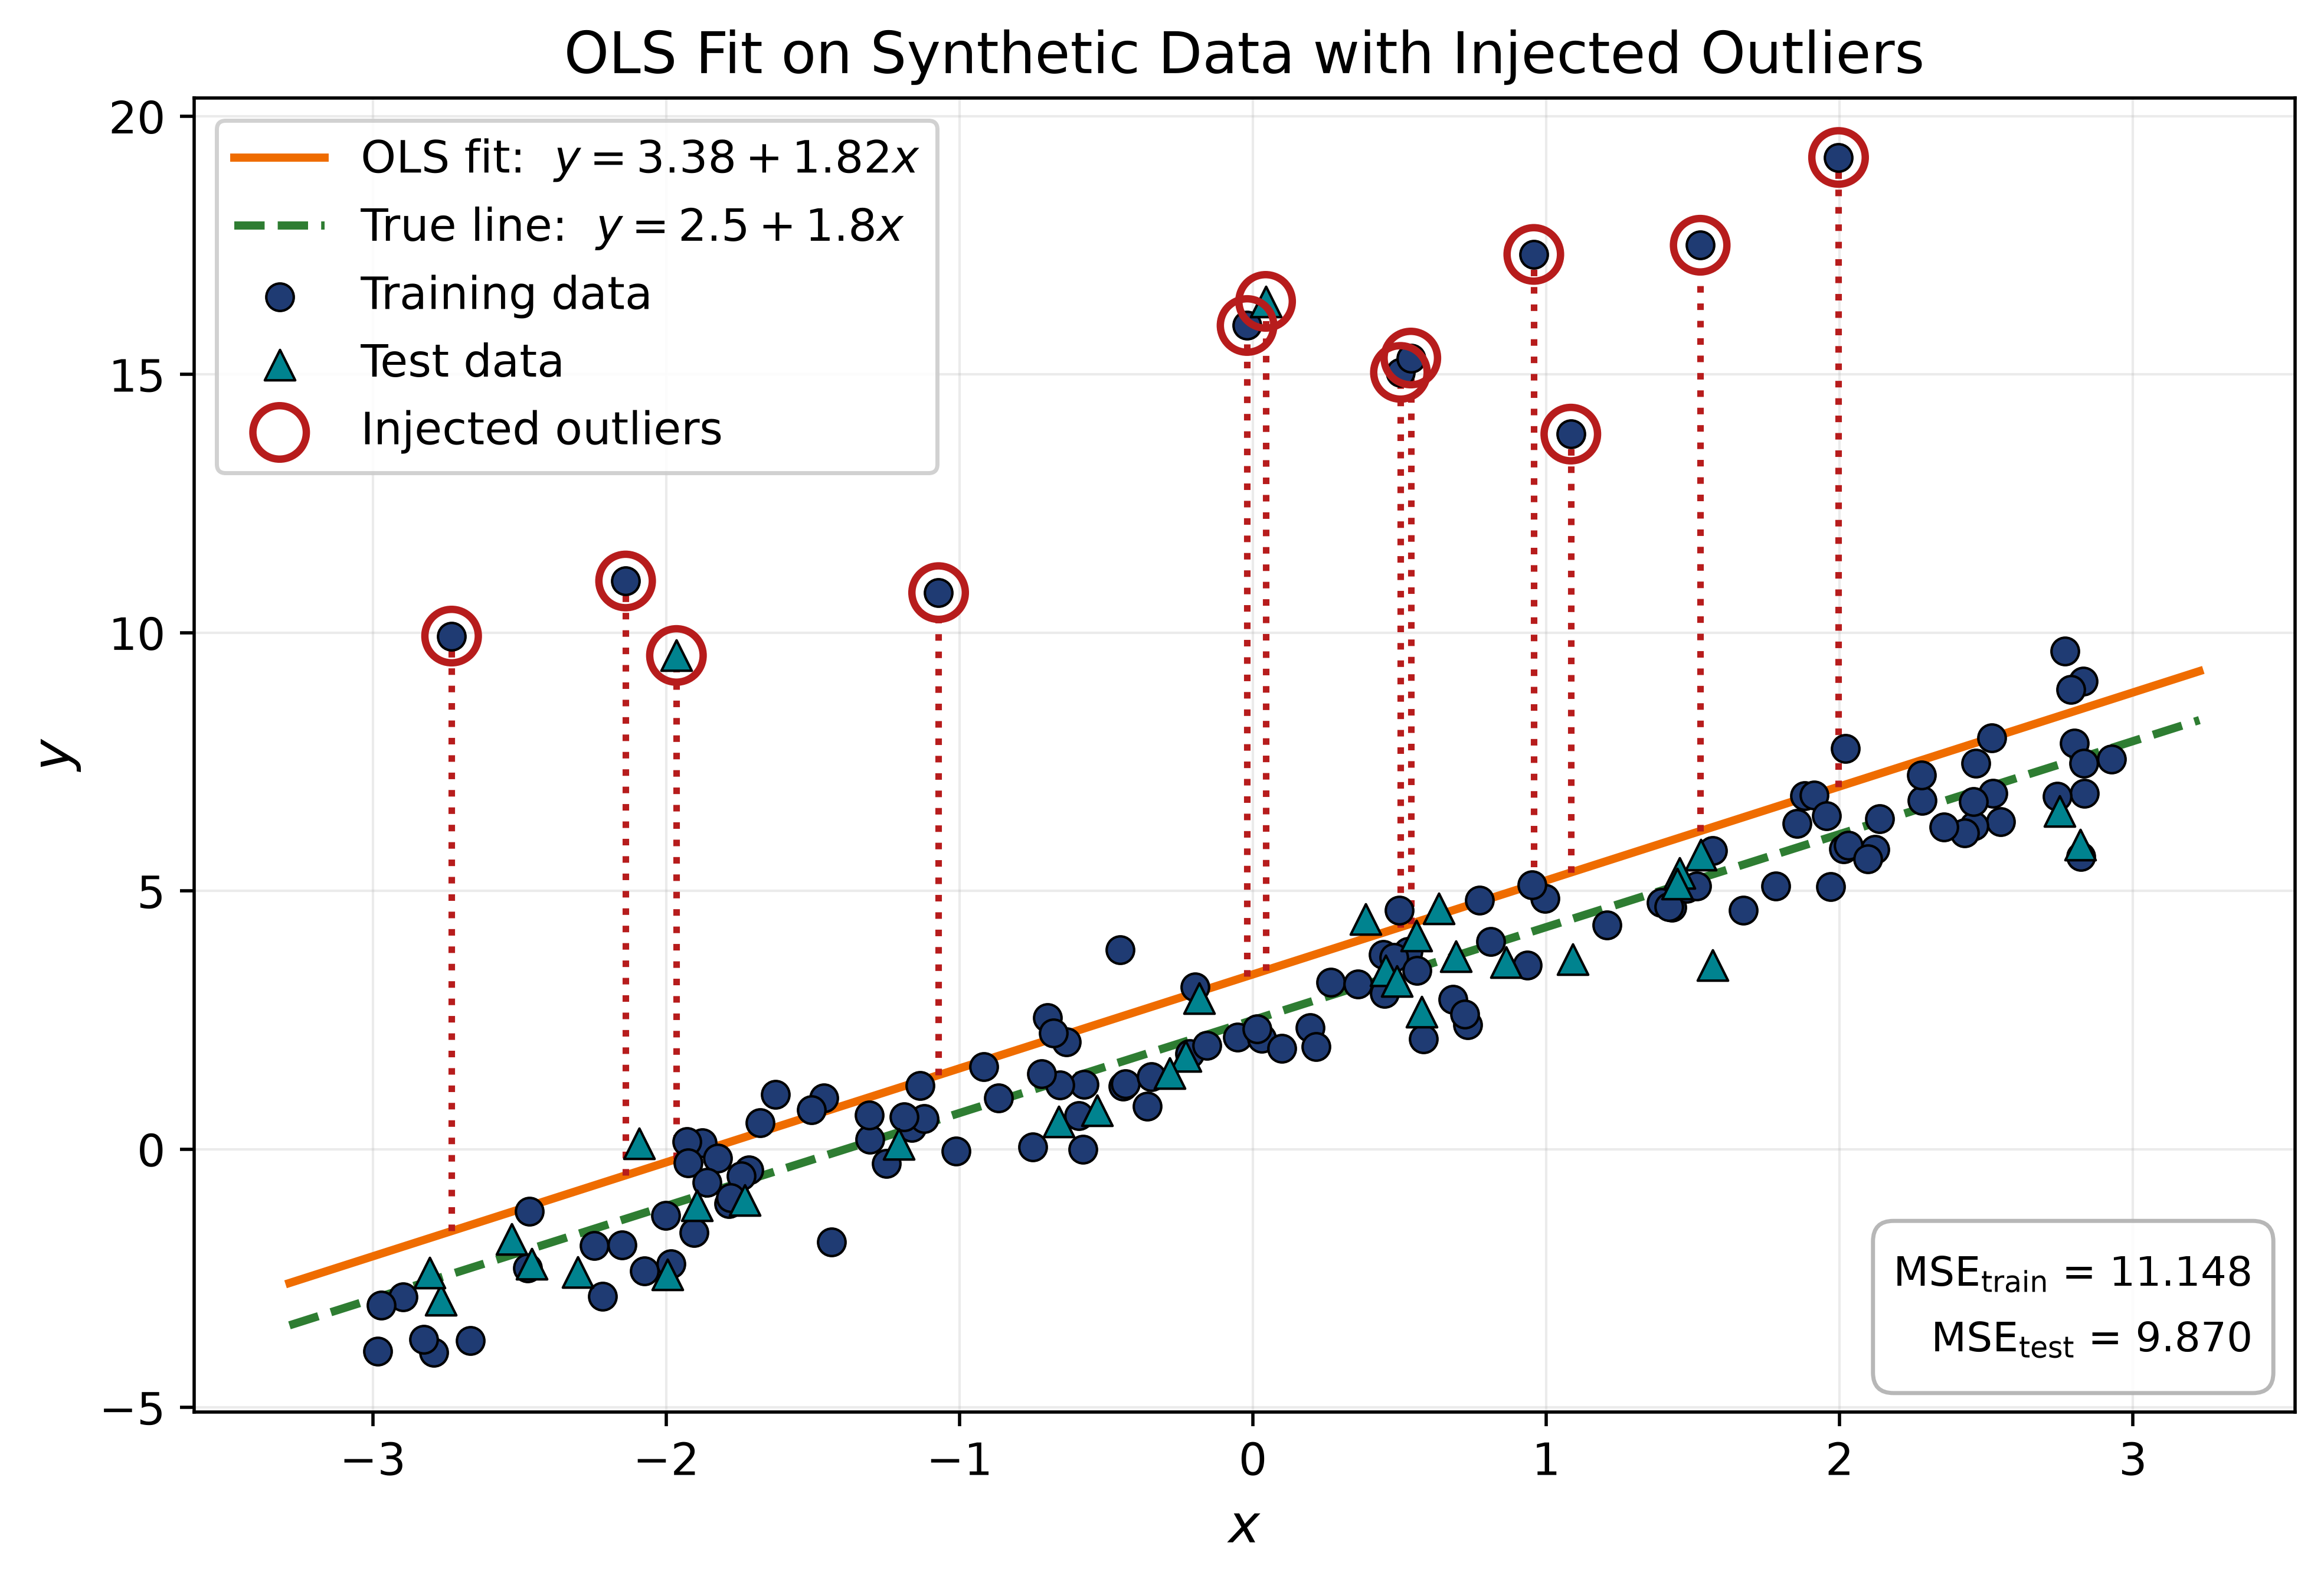
\includegraphics[width=0.88\textwidth]{figures/q1_2_ols_fit_outliers.png}
\caption{OLS fit on the synthetic data. The dotted vertical segments mark the residual of each
injected outlier against the fitted line.}
\label{fig:olsfit}
\end{figure}

The fitted intercept of 3.3842 sits well above the true value of 2.5, while the slope 1.8197
remains close to the true 1.8. This is the expected signature of purely vertical contamination:
the twelve upward shifts raise the fitted line bodily rather than tilting it.

\subsection{Weighted Least Squares}

\qtext{Define $a_i \in (0,1]$ as the sample-specific weight, where $a_i = 0.05$ for the known
outliers and $a_i = 1.0$ for all inliers. Derive the closed-form matrix expression for the
weighted least-squares estimator
$\hat{\boldsymbol{w}}_{\mathrm{WLS}} = (\boldsymbol{X}^T\boldsymbol{A}\boldsymbol{X})^{-1}
\boldsymbol{X}^T\boldsymbol{A}\boldsymbol{y}$. Implement this WLS estimator using NumPy and
compare its fitted line against standard OLS.}

\textbf{Weighted Least Squares}

We have

\begin{equation}
J(\mathbf{w}) = \frac{1}{2N}(\mathbf{y}-\mathbf{Xw})^T \mathbf{A} (\mathbf{y}-\mathbf{Xw})
\label{eq:wlsobj}
\end{equation}

where $\mathbf{A}$ is a diagonal matrix containing the weights $\alpha_i$. The known outliers have
weight $0.05$, while the inliers have weight $1.0$.

\textbf{1. Expanding the objective}

Expanding the quadratic expression,

\begin{equation*}
J(\mathbf{w}) = \frac{1}{2N}\left[
\mathbf{y}^T\mathbf{A}\mathbf{y}
-\mathbf{y}^T\mathbf{A}\mathbf{Xw}
-\mathbf{w}^T\mathbf{X}^T\mathbf{A}\mathbf{y}
+\mathbf{w}^T\mathbf{X}^T\mathbf{A}\mathbf{Xw}
\right].
\end{equation*}

Since $\mathbf{A}$ is diagonal, it is symmetric. The two middle terms are scalars and are equal,
so this becomes

\begin{equation*}
J(\mathbf{w}) = \frac{1}{2N}\left[
\mathbf{y}^T\mathbf{A}\mathbf{y}
-2\mathbf{w}^T\mathbf{X}^T\mathbf{A}\mathbf{y}
+\mathbf{w}^T\mathbf{X}^T\mathbf{A}\mathbf{Xw}
\right].
\end{equation*}

\textbf{2. Gradient}

Taking the derivative with respect to $\mathbf{w}$,

\begin{equation*}
\nabla_{\mathbf{w}}J = \frac{1}{2N}\left[
-2\mathbf{X}^T\mathbf{A}\mathbf{y} + 2\mathbf{X}^T\mathbf{A}\mathbf{Xw}\right].
\end{equation*}

Therefore,

\begin{equation}
\nabla_{\mathbf{w}}J = \frac{1}{N}\left(
\mathbf{X}^T\mathbf{A}\mathbf{Xw} - \mathbf{X}^T\mathbf{A}\mathbf{y}\right).
\label{eq:wlsgrad}
\end{equation}

\textbf{3. Setting the gradient to zero}

For the minimum, we set the gradient equal to zero:

\begin{equation}
\mathbf{X}^T\mathbf{A}\mathbf{X}\hat{\mathbf{w}} = \mathbf{X}^T\mathbf{A}\mathbf{y}.
\label{eq:wlsnormal}
\end{equation}

These are the weighted normal equations.

\textbf{4. Solving for $\hat{\mathbf{w}}$}

All the weights $\alpha_i$ are positive, so $\mathbf{A}$ is positive definite. Assuming that
$\mathbf{X}$ has full column rank, $\mathbf{X}^T\mathbf{A}\mathbf{X}$ is invertible.

Thus,

\begin{equation}
\hat{\mathbf{w}}_{\mathrm{WLS}} =
(\mathbf{X}^T\mathbf{A}\mathbf{X})^{-1}\mathbf{X}^T\mathbf{A}\mathbf{y}.
\label{eq:wls}
\end{equation}

\textbf{5. Checking the minimum}

The Hessian is

\begin{equation*}
\nabla_{\mathbf{w}}^2 J = \frac{1}{N}\mathbf{X}^T\mathbf{A}\mathbf{X}.
\end{equation*}

Since $\mathbf{X}^T\mathbf{A}\mathbf{X}$ is positive definite, the Hessian is also positive
definite. Therefore, the stationary point is the unique global minimum of $J(\mathbf{w})$.

Hence, the weighted least-squares solution is

\begin{equation*}
\hat{\mathbf{w}}_{\mathrm{WLS}} =
(\mathbf{X}^T\mathbf{A}\mathbf{X})^{-1}\mathbf{X}^T\mathbf{A}\mathbf{y}.
\end{equation*}

\lstinputlisting[caption={NumPy implementation of the OLS and WLS closed-form estimators.},
                 label={lst:wls}]{code/1_3_wls.py}

\begin{table}[H]
\centering
\caption{OLS against WLS with $a_i = 0.05$ on the known outliers. The inlier-only test MSE
excludes the two contaminated test rows.}
\label{tab:wls}
\begin{tabular}{lccccc}
\toprule
\textbf{Model} & $w_0$ & $w_1$ & \textbf{MSE}$_{\text{train}}$ & \textbf{MSE}$_{\text{test}}$
& \textbf{MSE}$_{\text{test}}$ \textbf{(inliers)} \\
\midrule
OLS   & 3.3842 & 1.8197 & 11.1480 & 9.8696  & 1.7663 \\
WLS   & 2.4926 & 1.8394 & 11.9395 & 10.1487 & 0.6348 \\
True  & 2.5000 & 1.8000 & --      & --      & --     \\
\bottomrule
\end{tabular}
\end{table}

\begin{lstlisting}[style=plainout]
Outliers in training set: 10 / 128
Outliers in test set    : 2 / 32

Euclidean distance from the true parameters [2.5, 1.8]:
  ||w_ols - w_true|| = 0.8844
  ||w_wls - w_true|| = 0.0401
\end{lstlisting}

\lstinputlisting[caption={Plotting the WLS and OLS fitted lines against the true line.},
                 label={lst:wlsplot}]{code/1_3_plot.py}

\begin{figure}[H]
\centering
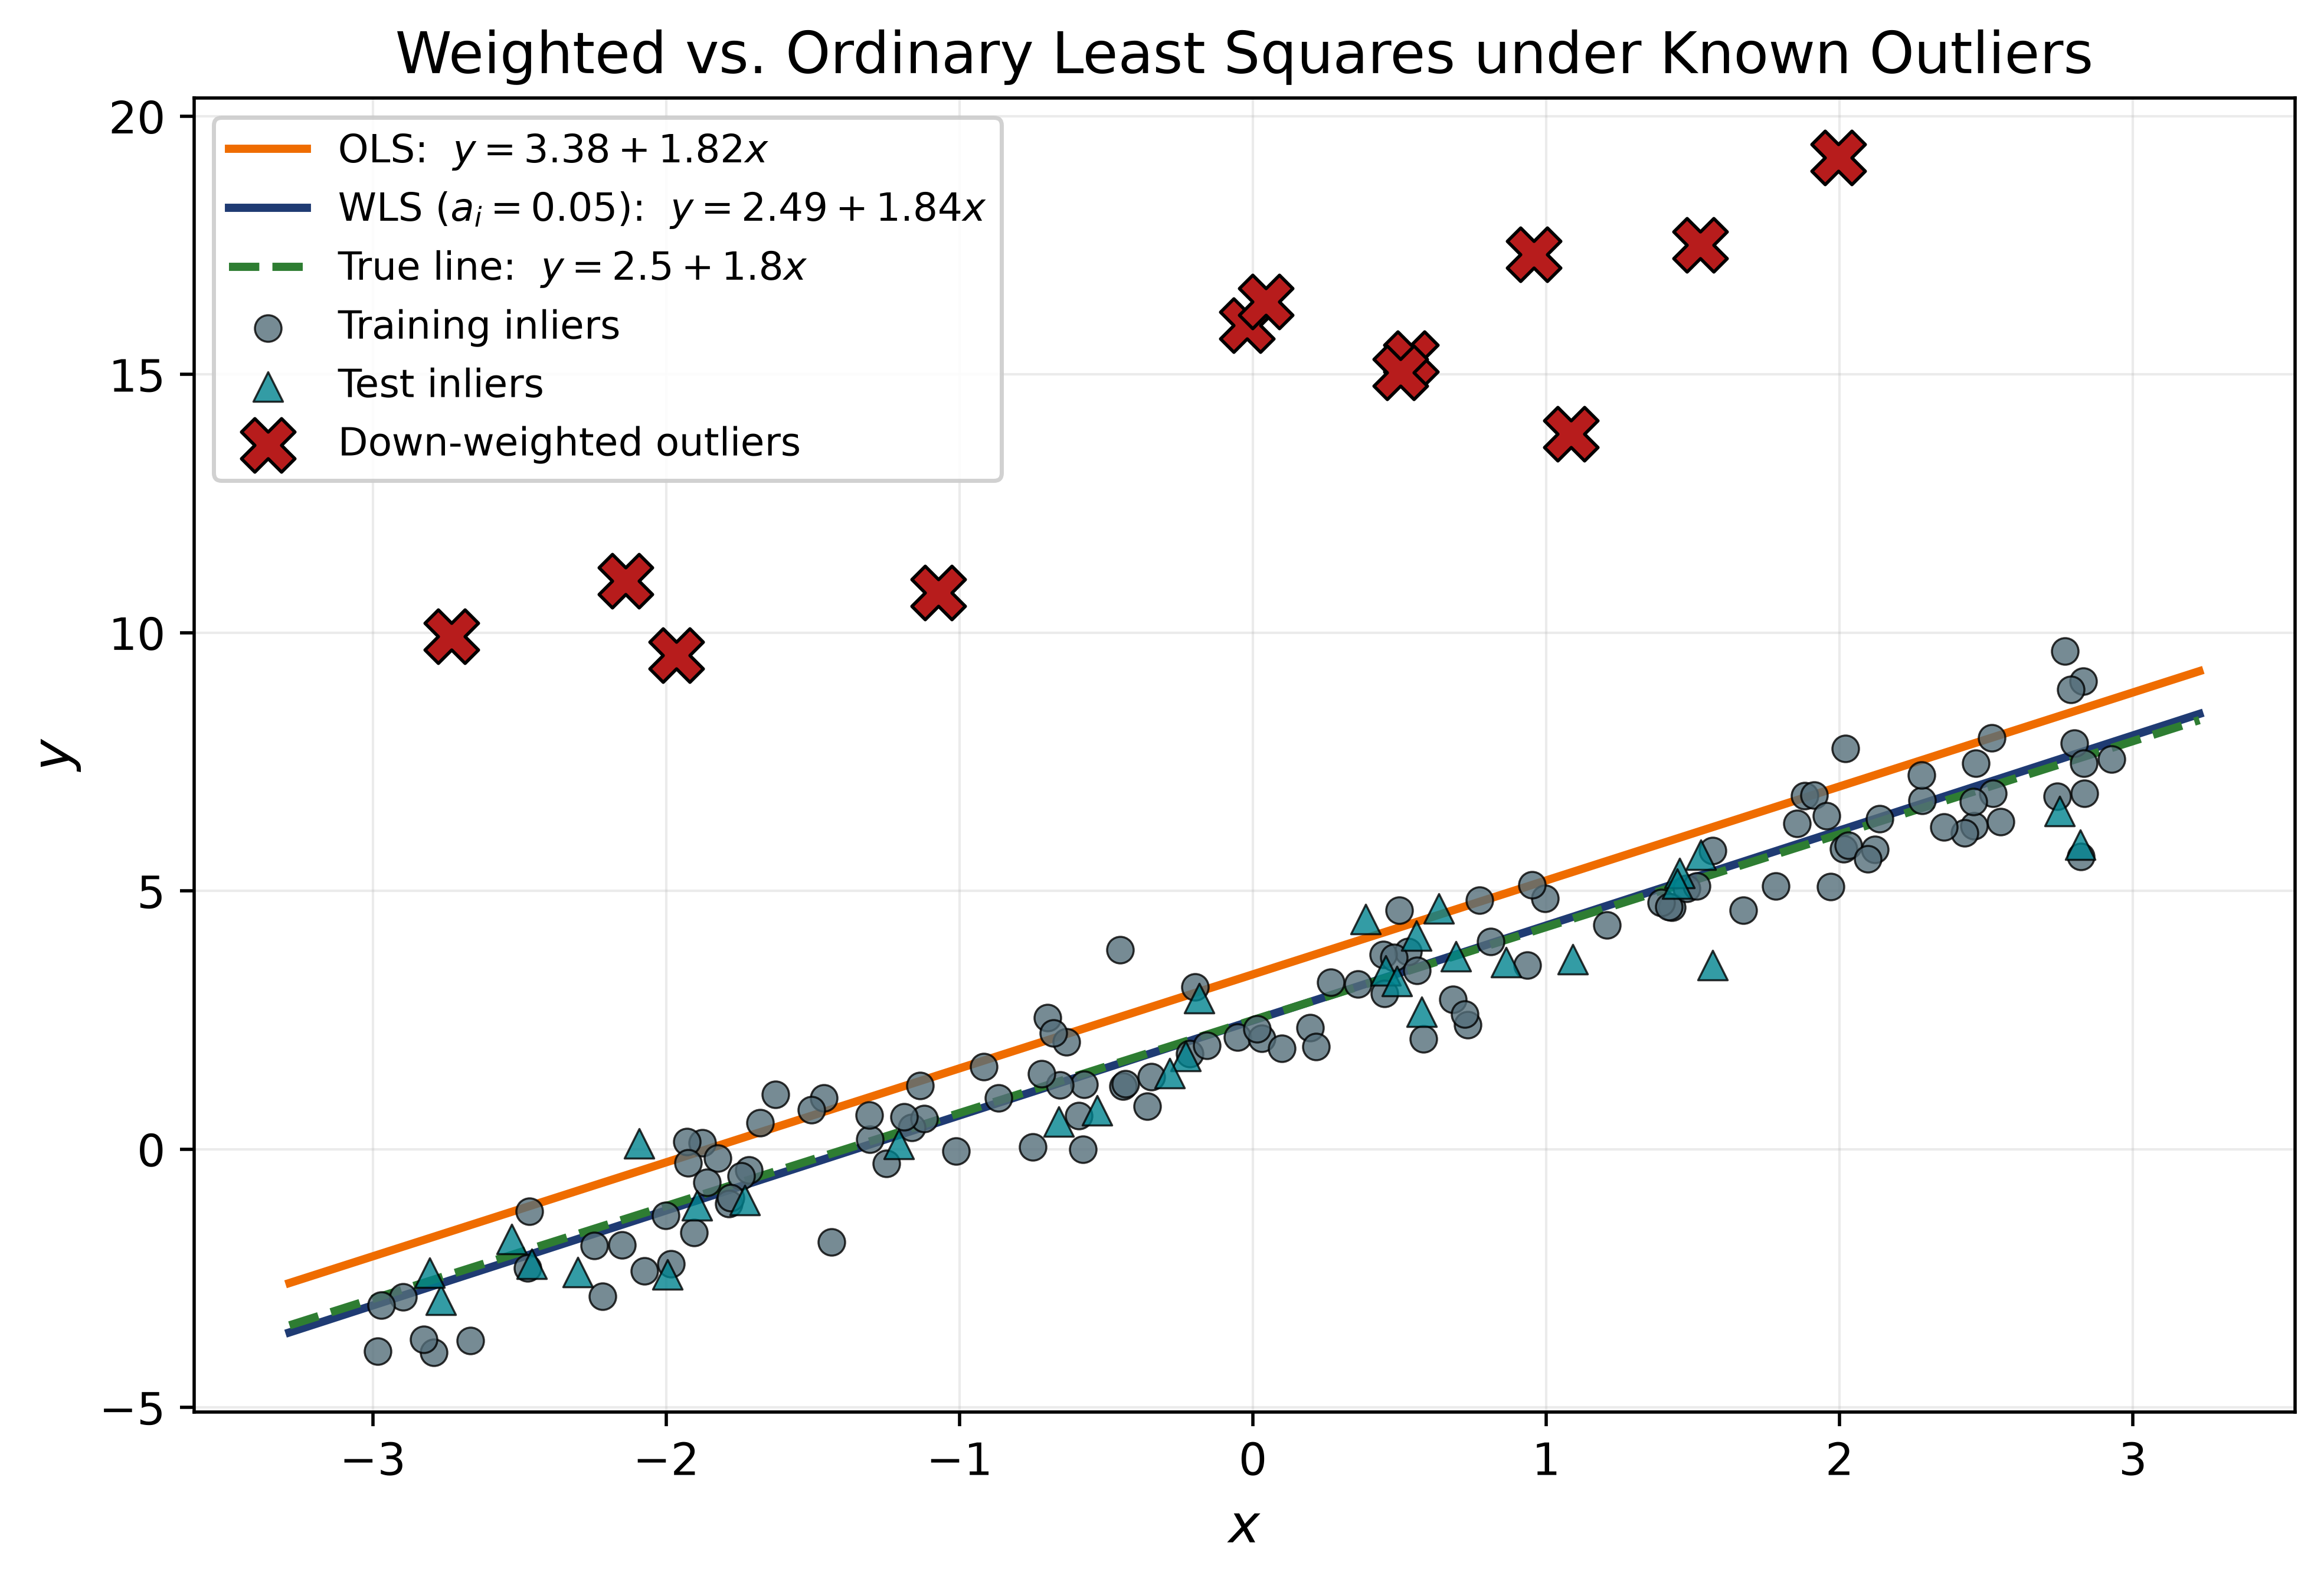
\includegraphics[width=0.88\textwidth]{figures/q1_3_wls_vs_ols.png}
\caption{Weighted against ordinary least squares under known outliers. Down-weighting the twelve
contaminated points recovers a line almost coincident with the true one.}
\label{fig:wlsfit}
\end{figure}

Down-weighting the known outliers by a factor of twenty recovers an intercept of 2.4926 against
the true 2.5, and reduces the distance from the true parameter vector from 0.8844 to 0.0401. The
overall test MSE is marginally worse for WLS, because that metric is dominated by the two
contaminated test rows the estimator deliberately discounts; on the inliers alone the test MSE
falls from 1.7663 to 0.6348.

\subsection{Regularization in High Dimensions}

\qtext{Create an expanded dataset containing nine pure noise variables. Fit OLS, Ridge Regression
($L_2$), and Lasso Regression ($L_1$). Tune the regularization strength hyperparameter
$\alpha \in \{10^{-3}, 10^{-2}, 10^{-1}, 1, 10\}$ using 5-fold cross-validation. Report optimal
$\alpha^*$ values and cross-validated test MSEs.}

\lstinputlisting[caption={OLS, Ridge and Lasso on one informative feature plus nine pure-noise
features, with $\alpha$ tuned by 5-fold cross-validation.},
                 label={lst:reg}]{code/1_4_regularization.py}

\begin{table}[H]
\centering
\caption{Optimal regularization strengths and cross-validated errors on the expanded
ten-feature dataset.}
\label{tab:reg}
\begin{tabular}{lcccc}
\toprule
\textbf{Model} & $\boldsymbol{\alpha^*}$ & \textbf{CV MSE} & \textbf{Test MSE}
& \textbf{Noise coefs}\ $\mathbf{= 0}$ \\
\midrule
OLS   & --  & 14.0434 & 10.3007 & 0 / 9 \\
Ridge & 10  & 13.7966 & 10.0921 & 0 / 9 \\
Lasso & 1   & 12.3842 & 10.1284 & 9 / 9 \\
\bottomrule
\end{tabular}
\end{table}

\begin{lstlisting}[style=plainout]
Fitted coefficients (feature 0 is the real one, 1-9 are pure noise):
               0       1       2       3       4       5       6       7       8       9
OLS        3.165  -0.026   0.070  -0.078  -0.157  -0.486   0.150  -0.329   0.062  -0.332
Ridge      2.922  -0.008   0.057  -0.055  -0.128  -0.419   0.138  -0.295   0.078  -0.331
Lasso      2.111   0.000   0.000   0.000   0.000   0.000   0.000   0.000   0.000   0.000
\end{lstlisting}

\lstinputlisting[caption={Bar chart of the fitted coefficients across the ten features.},
                 label={lst:regplot}]{code/1_4_plot.py}

\begin{figure}[H]
\centering
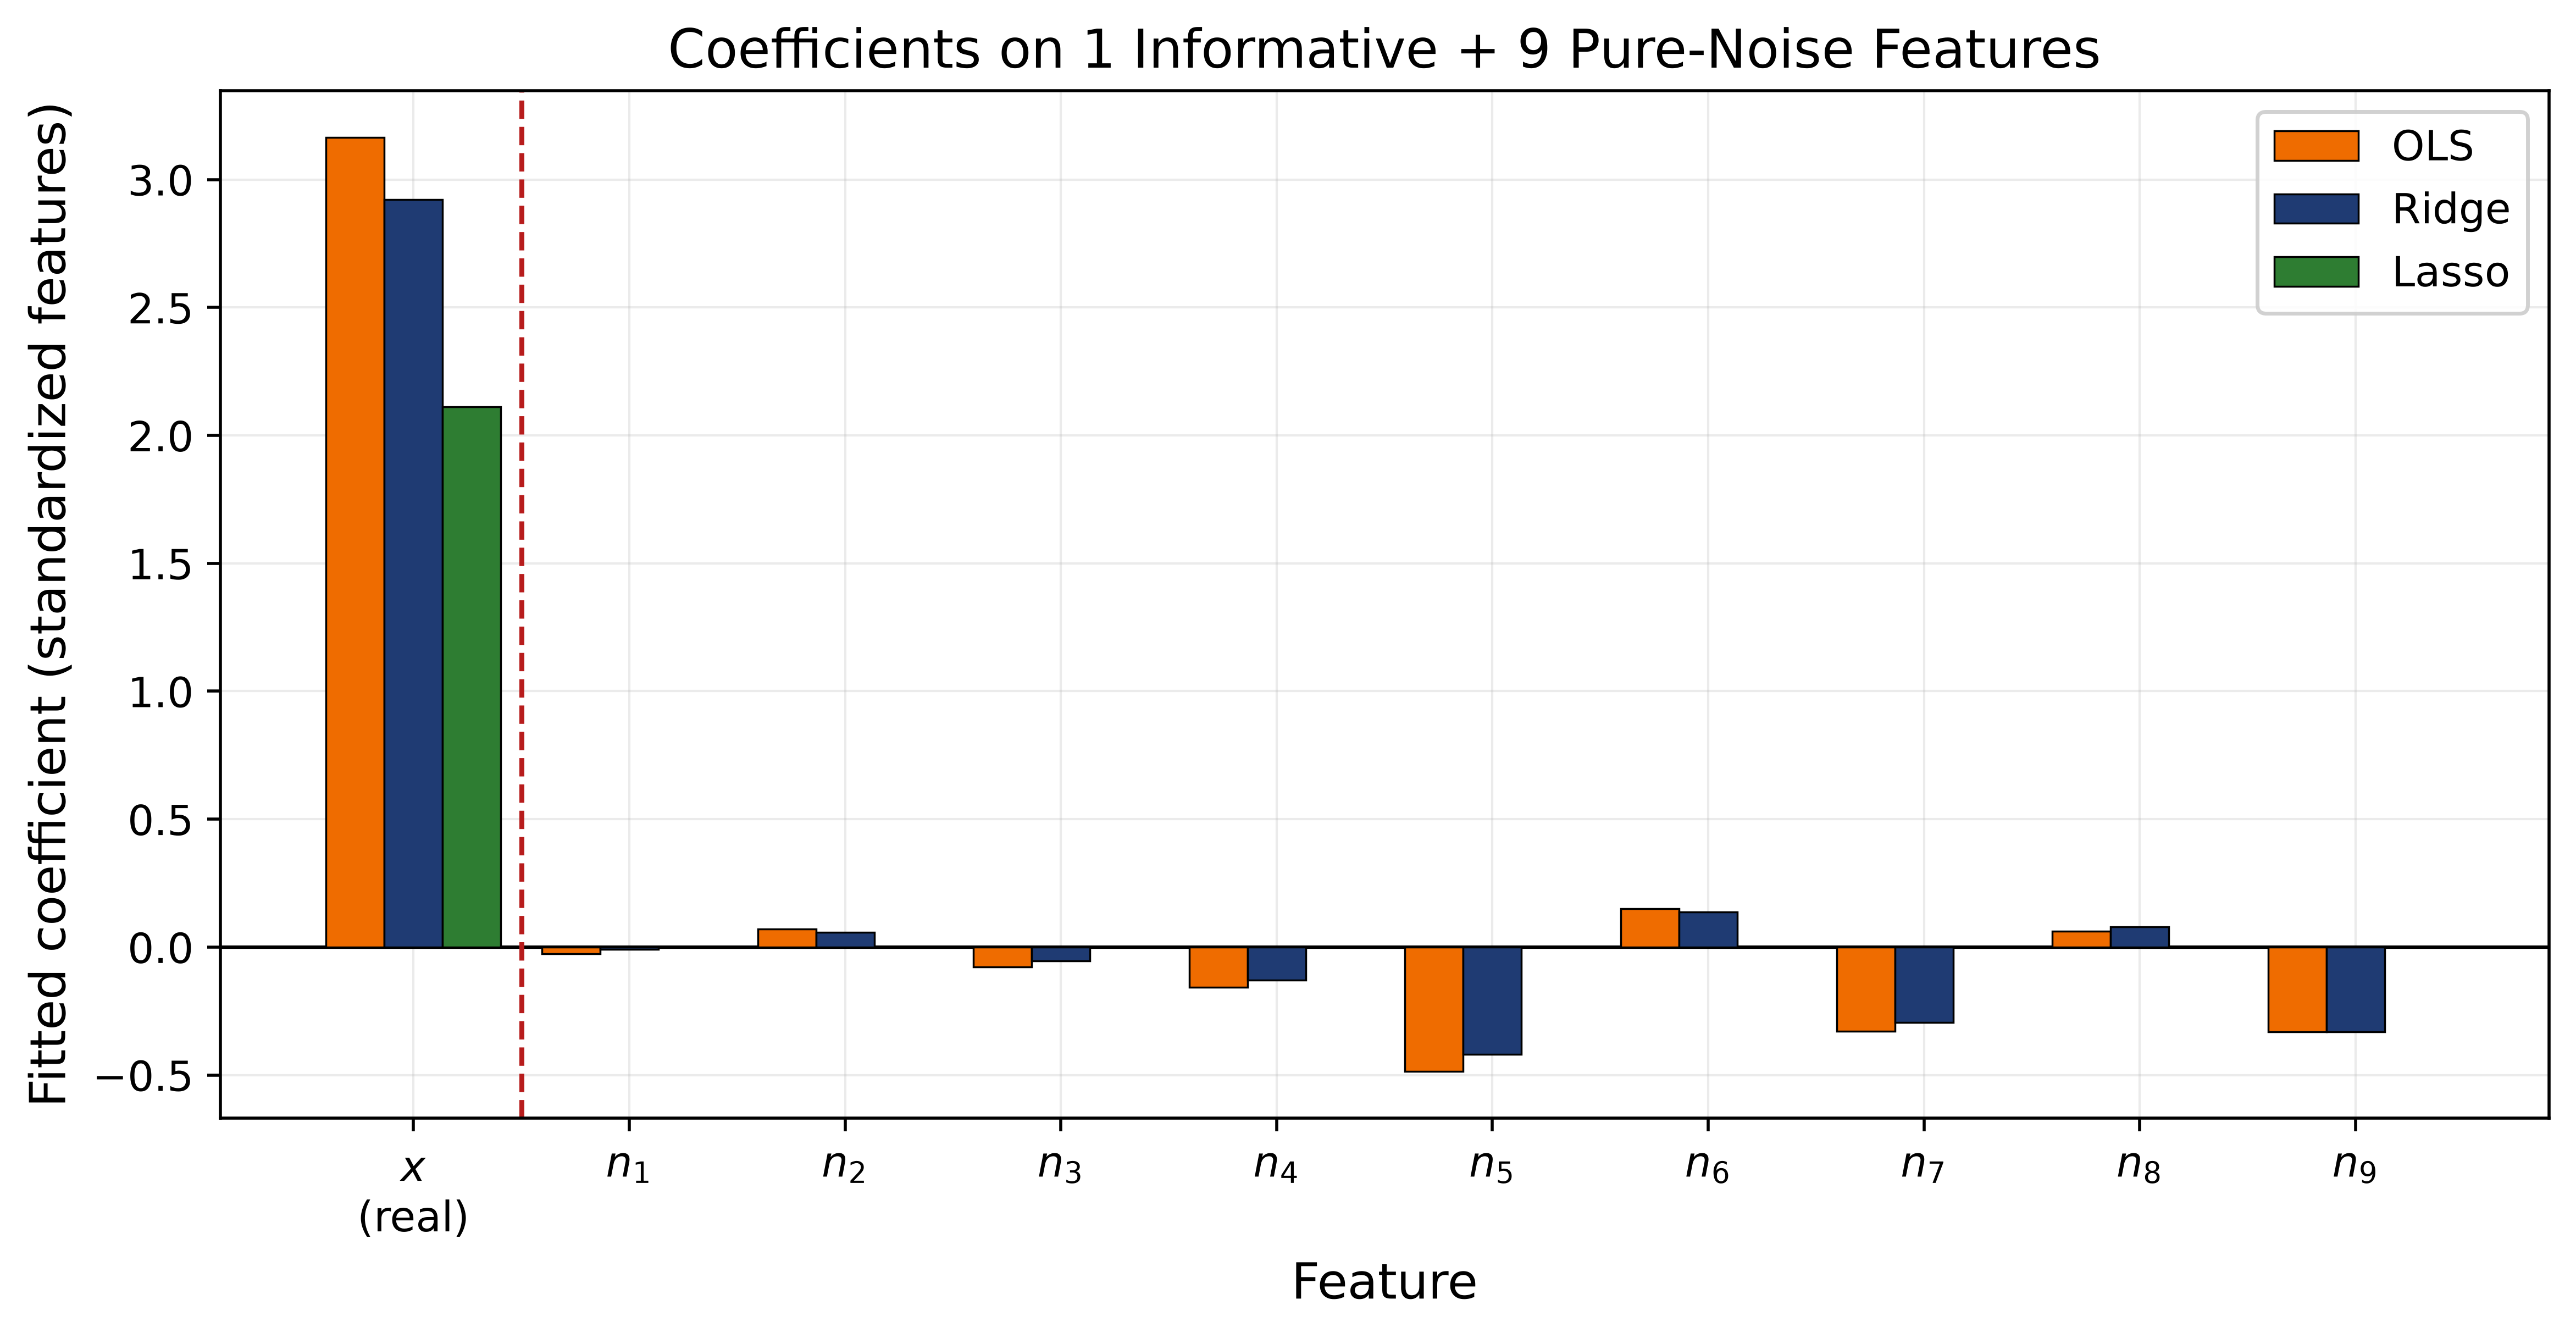
\includegraphics[width=0.95\textwidth]{figures/q1_4_coefficients.png}
\caption{Fitted coefficients on one informative and nine pure-noise features. Lasso eliminates
every noise coefficient exactly; Ridge shrinks them but retains all nine.}
\label{fig:coefs}
\end{figure}

\subsection{Ridge against Lasso}

\qtext{Compare Ridge and Lasso in terms of their mathematical penalty terms
($\|\boldsymbol{w}\|_2^2$ vs.\ $\|\boldsymbol{w}\|_1$), resulting coefficient magnitudes, and
capacity for sparse feature selection. Explain which model is preferable when $D \gg N$ and only a
small subset of features are genuinely informative.}

Ridge and Lasso both add a penalty to the loss function, but they affect the model coefficients in
different ways.

Ridge uses the $L_2$ penalty:

\begin{equation}
\alpha \|\mathbf{w}\|_2^2 = \alpha \sum_j w_j^2
\label{eq:l2}
\end{equation}

This penalty is smooth and differentiable. Lasso uses the $L_1$ penalty:

\begin{equation}
\alpha \|\mathbf{w}\|_1 = \alpha \sum_j |w_j|
\label{eq:l1}
\end{equation}

The $L_1$ penalty is not differentiable at $w_j=0$.

For an orthonormal design where

\begin{equation*}
\mathbf{X}^T\mathbf{X}=\mathbf{I},
\end{equation*}

and $\rho_j$ is the OLS coefficient, Ridge gives

\begin{equation}
\hat{w}_j=\frac{\rho_j}{1+\lambda}.
\label{eq:ridgeshrink}
\end{equation}

Therefore, Ridge shrinks all the coefficients towards zero by the same factor. But the
coefficients normally do not become exactly zero.

For Lasso, the solution is

\begin{equation}
\hat{w}_j = \operatorname{sign}(\rho_j)\max\left(|\rho_j|-\frac{\lambda}{2},0\right).
\label{eq:softthresh}
\end{equation}

If the value of $|\rho_j|$ is smaller than or equal to $\lambda/2$, the coefficient becomes
exactly zero.

The difference can also be understood geometrically. The $L_2$ constraint gives a round constraint
region, so the loss contours usually touch it at a point where most coefficients are nonzero. The
$L_1$ constraint has corners along the axes, making it more likely for the optimum to occur where
some coefficients are exactly zero.

Therefore, Lasso can automatically perform feature selection, while Ridge mainly shrinks the
coefficients.

When $D \gg N$ and only a few features are actually informative, I would prefer Lasso. Since most
of the features are irrelevant, Lasso can set their coefficients to zero and produce a sparse
model. This also makes the model easier to interpret.

In our Q4 experiment, Lasso with the selected $\alpha^*$ kept only the true feature $x$ and set the
9 noise-feature coefficients to zero. Ridge, on the other hand, kept all 10 coefficients nonzero.
This matches the expected difference between the two methods.

So, for a high-dimensional dataset with only a few useful features, Lasso is generally more
suitable because it can both reduce the effect of irrelevant features and select the important
ones.

\subsection{Necessity of Standardized Feature Scaling}

\qtext{Explain analytically why standardized feature scaling ($z = \frac{x-\mu}{\sigma}$) is
mandatory prior to penalizing weights in Ridge or Lasso regression.}

Feature scaling is important before applying Ridge or Lasso because the regularization penalty is
applied directly to the model weights. If the features have very different scales, the weights can
also have very different magnitudes even when the features are equally important.

Suppose a feature $x_j$ is changed to a different unit:

\begin{equation*}
x_j' = c x_j
\end{equation*}

To keep the predictions the same, its coefficient has to change to

\begin{equation}
w_j' = \frac{w_j}{c}.
\label{eq:rescale}
\end{equation}

For Ridge, the penalty for this coefficient changes from

\begin{equation*}
\alpha w_j^2
\end{equation*}

to

\begin{equation*}
\alpha (w_j')^2 = \alpha\frac{w_j^2}{c^2}.
\end{equation*}

For Lasso, it changes from

\begin{equation*}
\alpha |w_j|
\end{equation*}

to

\begin{equation*}
\alpha |w_j'| = \alpha\frac{|w_j|}{c}.
\end{equation*}

Therefore, simply changing the units of a feature changes how strongly that feature is penalized.
A feature with a small numerical scale will usually need a larger coefficient, so it can receive a
stronger effective penalty. A feature with a large numerical scale can have a smaller coefficient
and will be penalized less.

This is especially important for Lasso because the penalty can make a coefficient exactly zero.
Therefore, the scale of a feature can affect whether that feature is selected or removed from the
model.

To avoid this problem, we standardize each feature using

\begin{equation}
z_j = \frac{x_j-\mu_j}{\sigma_j}.
\label{eq:zscore}
\end{equation}

After standardization, the features have approximately zero mean and unit variance. This puts them
on the same scale, so the same regularization parameter $\alpha$ can be applied fairly to all
coefficients.

Therefore, standardization is needed before Ridge or Lasso when the features have different
scales. It makes the effect of the regularization depend more on the actual importance of the
features rather than on their measurement units.

This is also why the Q4 pipelines use \texttt{StandardScaler} before applying Ridge and Lasso.

%=======================================================================
\section{Logistic Regression: Preprocessing, Interpretation, and Evaluation}
%=======================================================================

The classification dataset contains 600 samples with four numerical features, two nominal
categorical columns, deliberate class imbalance (68\,\% negative, 32\,\% positive), 3\,\% label
noise, and 25 missing entries in \texttt{x3}.

\lstinputlisting[caption={Generation of the classification dataset with mixed attributes and
missing values.}, label={lst:clsdata}]{code/2_0_data.py}

\subsection{String-Valued Columns and Label Encoding}

\qtext{Explain why passing string-valued columns directly to \texttt{LogisticRegression} throws a
runtime error. Furthermore, explain why applying basic \texttt{LabelEncoder} mapping categories to
integers $\{0,1,2\}$ introduces a spurious ordinal assumption that degrades model
generalizability.}

Logistic Regression cannot directly use string values such as \texttt{"north"}, \texttt{"south"},
\texttt{"east"}, \texttt{"mobile"}, or \texttt{"desktop"}. The model works with numerical values.
It first calculates a linear score

\begin{equation}
z = \mathbf{w}^T\mathbf{x} + b
\label{eq:linscore}
\end{equation}

and then applies the sigmoid function

\begin{equation}
p = \frac{1}{1+e^{-z}}
\label{eq:sigmoid2}
\end{equation}

Because of this, the input features need to be numerical. If string columns are given directly to
\texttt{LogisticRegression}, scikit-learn tries to convert the values into numbers. Values such as
\texttt{"north"} cannot be converted, so an error like the following can occur:

\begin{lstlisting}[style=plainout]
ValueError: could not convert string to float: 'north'
\end{lstlisting}

Using \texttt{LabelEncoder} is also not a good solution for nominal categorical features. For
example, suppose the \texttt{region} values are encoded as

\begin{lstlisting}[style=plainout]
east  -> 0
north -> 1
south -> 2
\end{lstlisting}

Logistic Regression would then treat these values as numerical quantities. This creates an
artificial ordering:

\begin{equation*}
\text{south} > \text{north} > \text{east}.
\end{equation*}

It also assumes that the distance between \texttt{east} and \texttt{north} is the same as the
distance between \texttt{north} and \texttt{south}.

There is no such relationship between these regions. They are nominal categories, so there is no
natural order or numerical distance between them. This is known as a spurious ordinal assumption.

Because of this, the model could learn patterns based on the arbitrary numbers assigned by
\texttt{LabelEncoder}. Also, changing the encoding, for example by assigning
\texttt{east -> 2} instead of \texttt{east -> 0}, could change the model even though the original
data has not changed.

\subsection{Preprocessing Pipeline and Stratified Split}

\qtext{Construct a scikit-learn \texttt{Pipeline} combined with \texttt{ColumnTransformer} that
imputes missing numerical entries with training set column medians; standardizes numerical
features ($\mu = 0$, $\sigma = 1$); imputes missing categorical features using the most frequent
mode; one-hot encodes categorical attributes; and fits a Logistic Regression classifier. Split the
dataset into training (80\,\%) and test (20\,\%) subsets using a stratified split with
\texttt{random\_state=42}.}

\lstinputlisting[caption={Preprocessing pipeline combining \texttt{ColumnTransformer} with
imputation, scaling, one-hot encoding and the classifier.},
                 label={lst:pipe}]{code/2_2_pipeline.py}

\begin{lstlisting}[style=plainout]
Train size: 480, test size: 120
Positive class share - train: 0.329, test: 0.325
Missing x3 values    - train: 22, test: 3

Features after preprocessing:
['num__x1', 'num__x2', 'num__x3', 'num__x4', 'cat__region_east',
 'cat__region_north', 'cat__region_south', 'cat__device_desktop',
 'cat__device_mobile']

Train accuracy: 0.8854
Test accuracy : 0.8500
\end{lstlisting}

Nesting the imputer inside the pipeline is what makes the medians training-set medians as the
question requires: the median is computed during \texttt{fit} on the 480 training rows and merely
applied to the test set, so no test information leaks into training. The stratified split holds
the positive-class share at 0.329 and 0.325 against the population rate of 0.328.

\subsection{Grid Search over Regularization Strength and Penalty}

\qtext{Perform a grid search over regularization strengths $C \in \{0.01, 0.1, 1, 10, 100\}$ and
penalty types penalty $\in \{\ell_1, \ell_2\}$ using \texttt{solver='liblinear'} and 5-fold
Stratified Cross-Validation. Optimize for $F_1$-score. Report best parameters and cross-validation
score.}

\lstinputlisting[caption={Grid search over $C$ and penalty type with 5-fold stratified
cross-validation, optimizing $F_1$.}, label={lst:grid}]{code/2_3_gridsearch.py}

\begin{table}[H]
\centering
\caption{Mean 5-fold cross-validated $F_1$-score for every combination in the grid.}
\label{tab:grid}
\begin{tabular}{lcc}
\toprule
$\boldsymbol{C}$ & $\boldsymbol{\ell_1}$ & $\boldsymbol{\ell_2}$ \\
\midrule
0.01 & 0.7418 & 0.7843 \\
0.1  & 0.8007 & 0.8033 \\
1    & \textbf{0.8148} & 0.8073 \\
10   & 0.7997 & 0.7997 \\
100  & 0.7997 & 0.7997 \\
\bottomrule
\end{tabular}
\end{table}

The best parameters are $C = 1$ with an $\ell_1$ penalty, giving a best cross-validated
$F_1$-score of \textbf{0.8148}. The scores at $C = 10$ and $C = 100$ are identical for both
penalties, indicating that regularization has effectively switched off at that strength and both
penalties converge to the same unconstrained solution.

\subsection{Test-Set Evaluation and Class Imbalance}

\qtext{On the test set, evaluate and report accuracy, precision, recall, $F_1$-score, and
confusion matrix. Explain why overall accuracy can be deeply misleading when dealing with
class-imbalanced datasets (e.g., 68\,\% negative, 32\,\% positive).}

\lstinputlisting[caption={Test-set evaluation of the tuned classifier.},
                 label={lst:metrics}]{code/2_4_metrics.py}

\lstinputlisting[caption={Rendering the confusion matrix.},
                 label={lst:cmplot}]{code/2_4_plot.py}

\textbf{Test-set results:}

\begin{table}[H]
\centering
\caption{Test-set performance of the tuned logistic regression model.}
\label{tab:metrics}
\begin{tabular}{lc}
\toprule
\textbf{Metric} & \textbf{Value} \\
\midrule
Accuracy  & 0.8583 \\
Precision & 0.7895 \\
Recall    & 0.7692 \\
F1-score  & 0.7792 \\
\bottomrule
\end{tabular}
\end{table}

Confusion matrix (rows = true, columns = predicted):

\begin{table}[H]
\centering
\caption{Confusion matrix on the 120 test samples.}
\label{tab:cm}
\begin{tabular}{lcc}
\toprule
 & \textbf{pred 0} & \textbf{pred 1} \\
\midrule
\textbf{true 0} & TN = 73 & FP = 8  \\
\textbf{true 1} & FN = 9  & TP = 30 \\
\bottomrule
\end{tabular}
\end{table}

\begin{figure}[H]
\centering
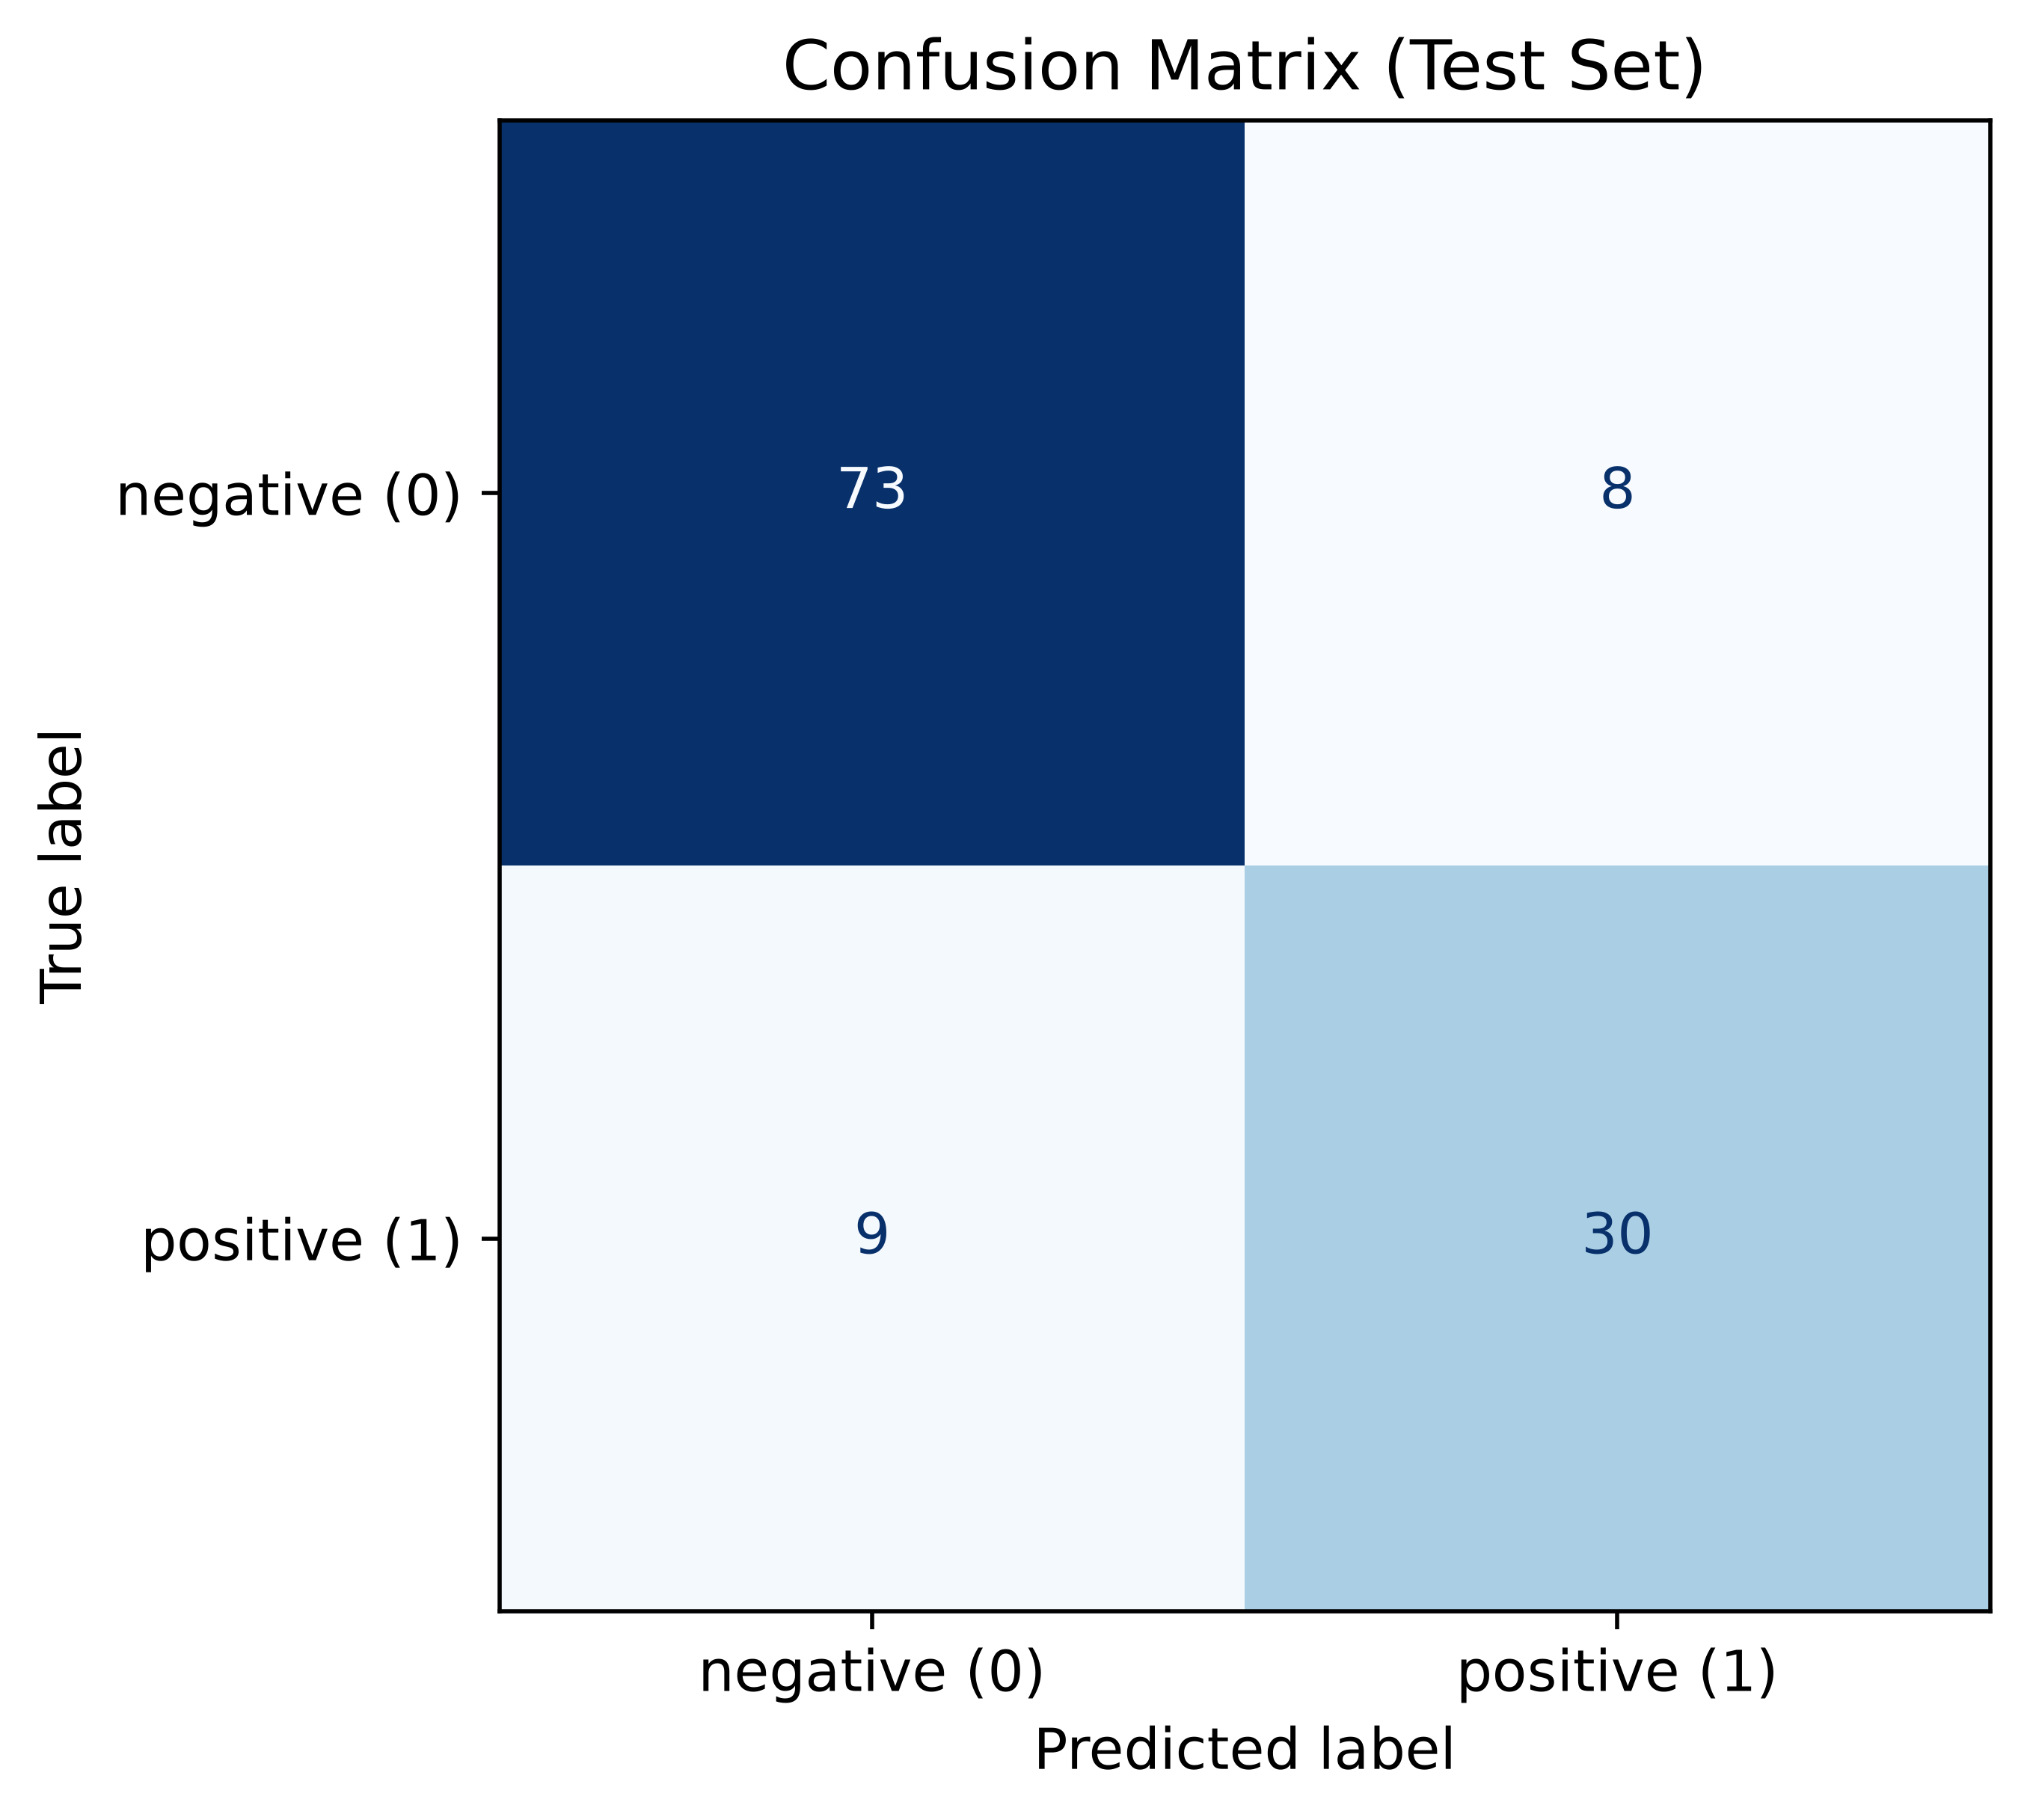
\includegraphics[width=0.56\textwidth]{figures/q2_4_confusion_matrix.png}
\caption{Confusion matrix of the tuned classifier on the test set.}
\label{fig:cm}
\end{figure}

Majority-class (always-0) baseline accuracy: \textbf{0.6750}.

\textbf{Why overall accuracy is misleading under class imbalance}

In this dataset, the classes are not balanced: about 68\,\% of the samples belong to the negative
class and 32\,\% belong to the positive class. Because of this, accuracy alone does not give a
good idea of how well the classifier is performing.

First, consider a very simple classifier that always predicts the majority class. There are 81
negative samples out of 120, so this classifier would get

\begin{equation}
\frac{81}{120}=0.675
\label{eq:baseline}
\end{equation}

Therefore, an accuracy of around 0.70 or even 0.80 does not necessarily mean that the model is
learning useful patterns.

Another problem is that the majority class has a large effect on the accuracy. Accuracy is
calculated as

\begin{equation}
\text{Accuracy}=\frac{TP+TN}{N}
\label{eq:accuracy}
\end{equation}

Since the negative class makes up most of the test set, getting the negative predictions correct
can make the accuracy look good. For example, a model that completely fails to detect the positive
class and has a recall of 0 could still get 67.5\,\% accuracy by predicting every sample as
negative.

Accuracy also treats false positives and false negatives in the same way. However, these two types
of errors may not have the same importance. For example, in medical diagnosis, missing a positive
case can be much more serious than incorrectly identifying a negative case as positive. Accuracy
does not show this difference.

For our model, the accuracy is 0.8583, which is much better than the 0.675 majority-class
baseline. The model correctly identifies 30 out of the 39 positive samples. However, imagine that
it detected only about 21 positive samples instead, with around 18 false negatives. The accuracy
would still be about

\begin{equation*}
\frac{21+(81-8)}{120} \approx 0.78,
\end{equation*}

while the positive-class recall would drop to

\begin{equation*}
\frac{21}{21+18} \approx 0.54.
\end{equation*}

So the accuracy would still look reasonably good even though the model would be missing almost
half of the positive cases.

Therefore, accuracy should not be used alone for this imbalanced dataset. Measures such as
precision, recall, F1-score, the confusion matrix, and ROC/PR curves give a better picture of the
model's performance. This is also why the hyperparameter search in Q2.3 used F1-score instead of
accuracy.

\subsection{Decision Threshold and the Precision-Recall Trade-off}

\qtext{Adjust the classification decision boundary threshold from $p_{\text{threshold}} = 0.50$
down to $0.35$. Recompute precision and recall. Describe the Precision-Recall trade-off and
outline a realistic domain application (e.g., medical diagnostics, fraud detection) where lowering
the threshold is preferred.}

\lstinputlisting[caption={Recomputing precision and recall at the lowered decision threshold.},
                 label={lst:thresh}]{code/2_5_threshold.py}

\begin{table}[H]
\centering
\caption{Effect of lowering the decision threshold from 0.50 to 0.35.}
\label{tab:thresh}
\begin{tabular}{lccccccc}
\toprule
\textbf{Threshold} & \textbf{Precision} & \textbf{Recall} & \textbf{F1}
& \textbf{TP} & \textbf{FP} & \textbf{FN} & \textbf{TN} \\
\midrule
0.50 & 0.7895 & 0.7692 & 0.7792 & 30 & 8  & 9 & 73 \\
0.35 & 0.6875 & 0.8462 & 0.7586 & 33 & 15 & 6 & 66 \\
\bottomrule
\end{tabular}
\end{table}

\begin{lstlisting}[style=plainout]
Precision change: 0.7895 -> 0.6875  (-0.1020)
Recall change   : 0.7692 -> 0.8462  (+0.0769)
\end{lstlisting}

\lstinputlisting[caption={Plotting the precision-recall curve with both operating points marked.},
                 label={lst:prplot}]{code/2_5_plot.py}

\begin{figure}[H]
\centering
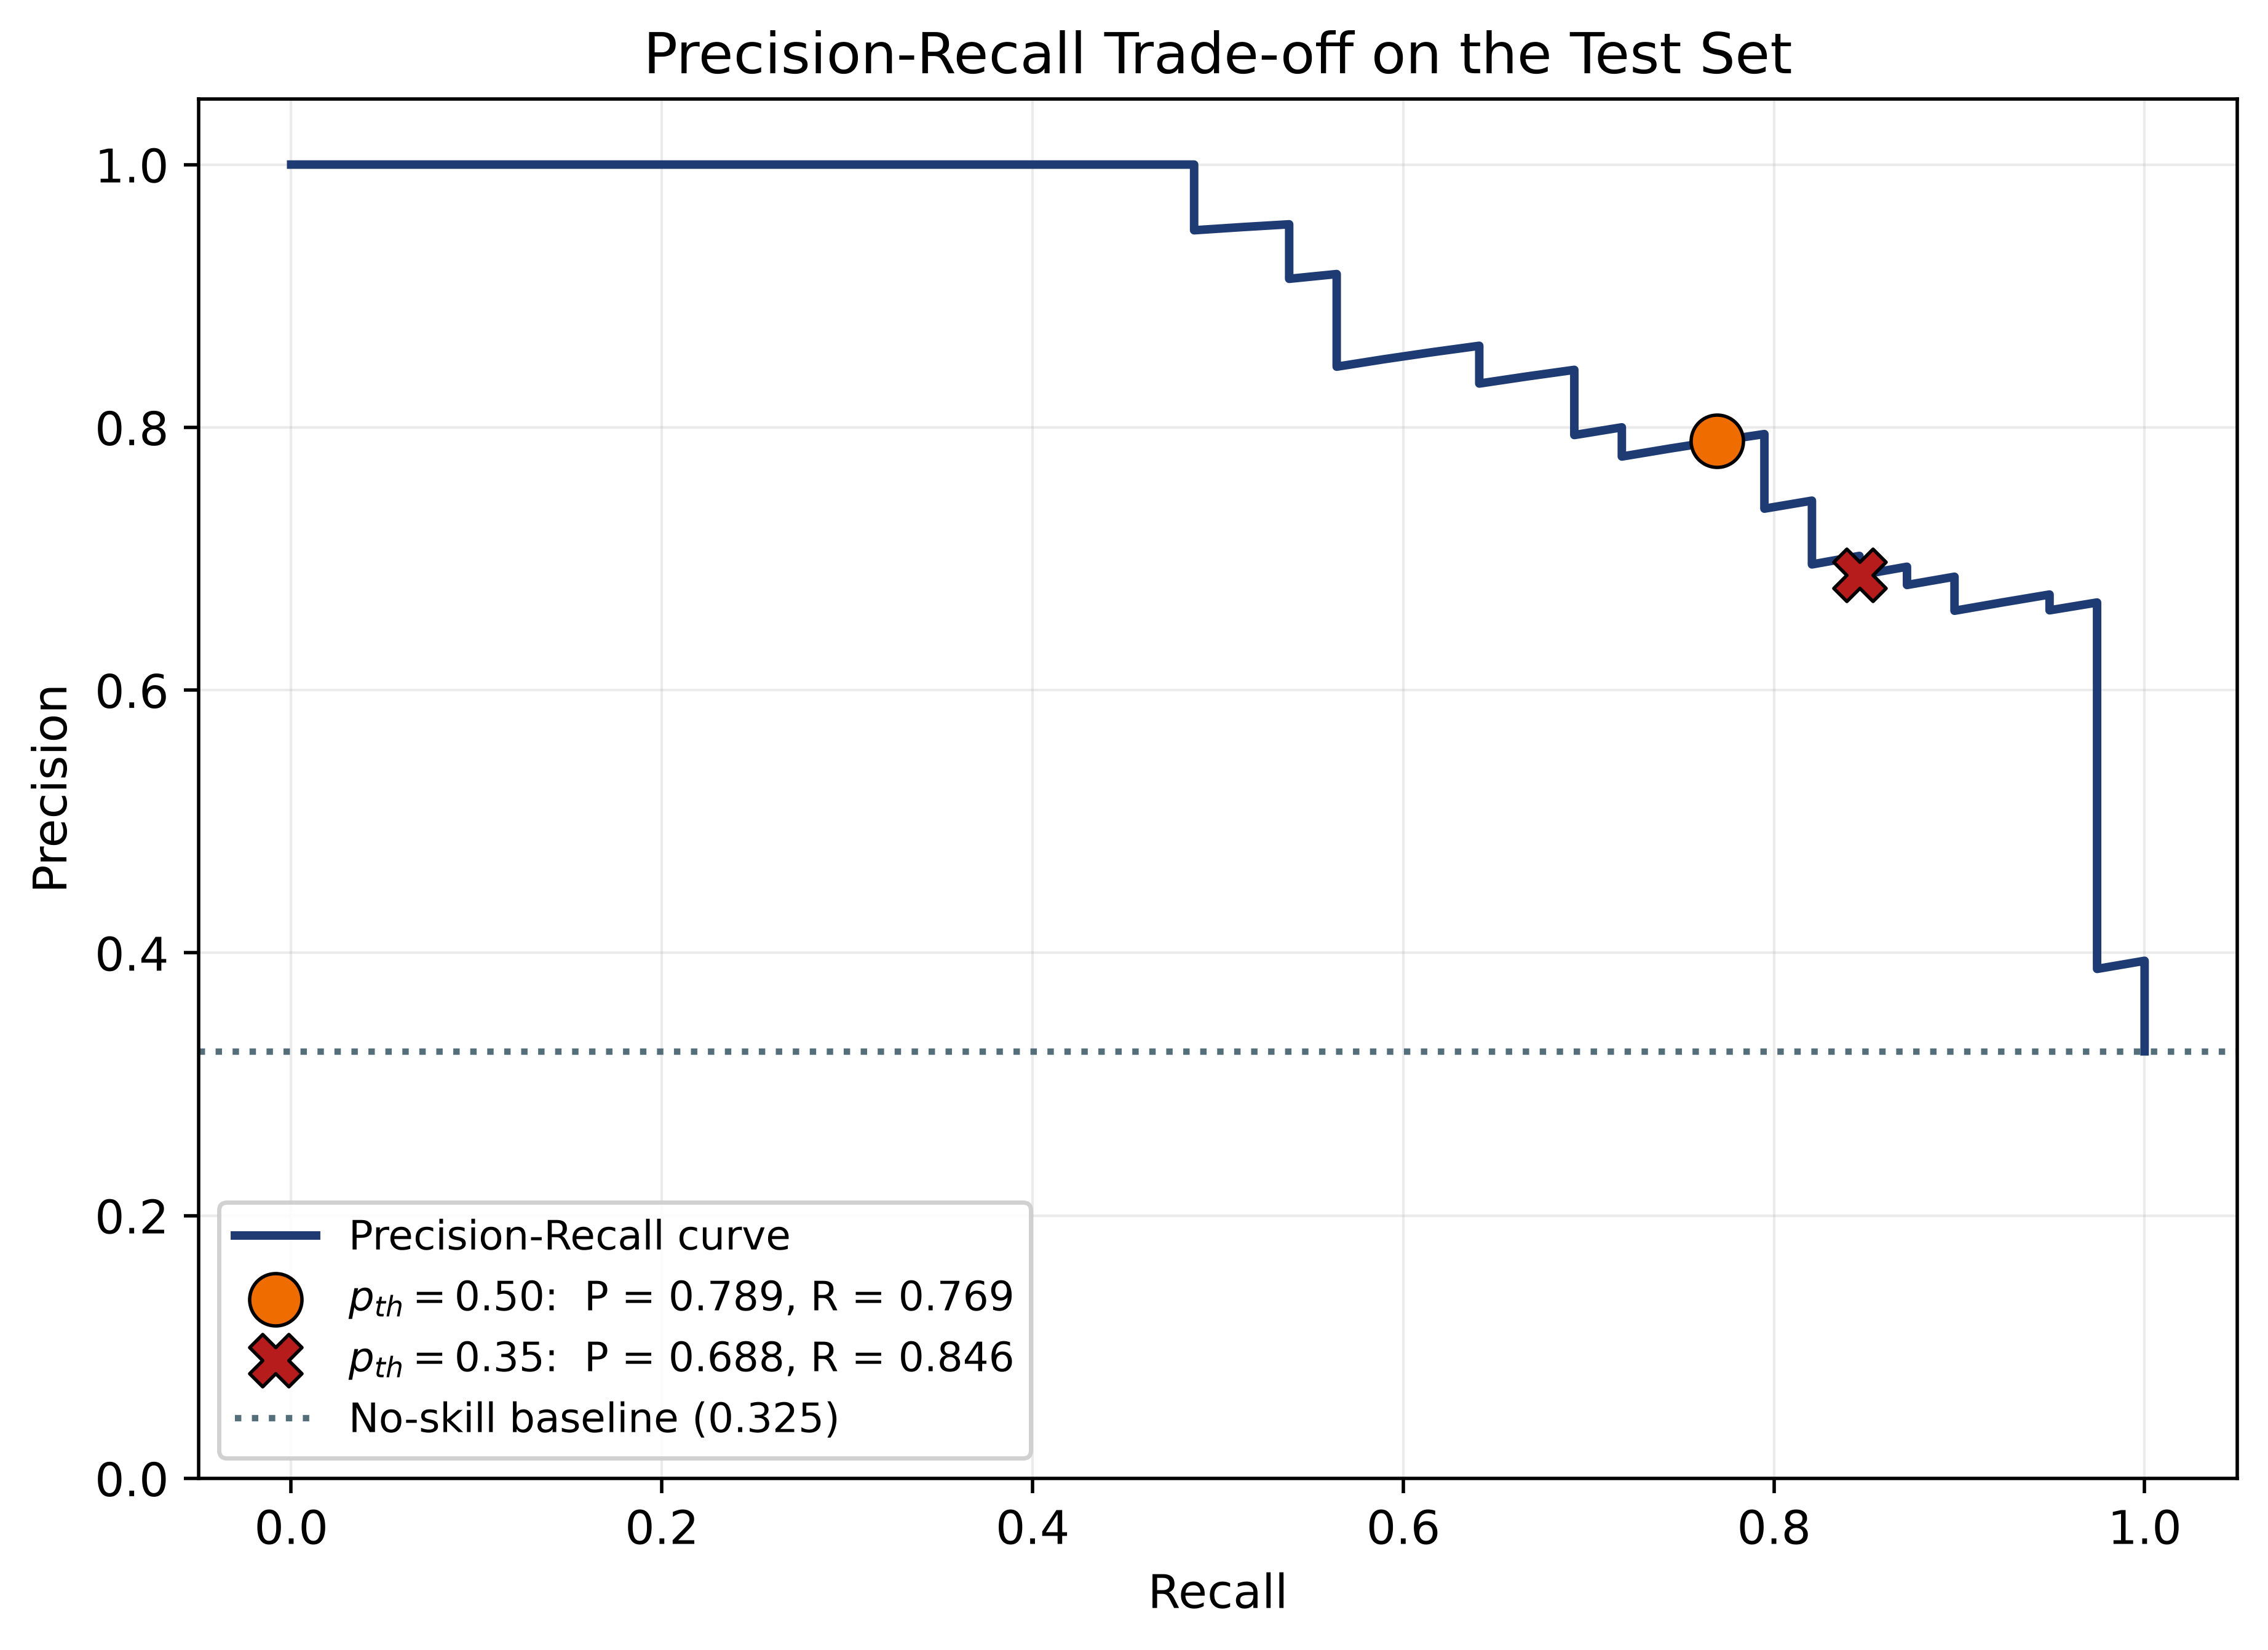
\includegraphics[width=0.86\textwidth]{figures/q2_5_precision_recall.png}
\caption{Precision-recall trade-off on the test set, with the $p_{th} = 0.50$ and $p_{th} = 0.35$
operating points marked.}
\label{fig:pr}
\end{figure}

When the threshold is reduced from 0.50 to 0.35, the model becomes less strict about predicting
the positive class. This means that more samples are classified as positive.

Because of this, the model can identify more of the actual positive samples, so recall increases.
However, some of the additional positive predictions will be incorrect, which causes precision to
decrease.

So there is a trade-off between precision and recall. In general, increasing recall means
accepting more false positives, which can reduce precision.

A good example is medical screening, such as detecting cancer or another serious disease. In this
situation, a false negative can be much more serious than a false positive. Missing a patient who
actually has the disease could delay treatment, while a false positive can usually be handled with
another test.

Therefore, in this type of application, it can be useful to lower the decision threshold. This
increases recall and helps reduce the number of patients who are missed, even though it also
produces more false alarms.

\subsection{Direct Probability Computation}

\qtext{A logistic regression model predicting whether a student passes with an $A^+$ ($y=1$)
yields $\ln\left(\frac{p}{1-p}\right) = -7.2 + 0.08x_1 + 1.4x_2$, where $x_1$ denotes study hours,
$x_2$ denotes GPA, and $p = P(y = 1\mid x)$. \textbf{(a)} Derive the sigmoid expression
$p = \frac{1}{1+e^{-z}}$ from logit $z = \ln\left(\frac{p}{1-p}\right)$. Calculate the probability
$p$ for a student with $x_1 = 45$ study hours and $x_2 = 3.4$ GPA. \textbf{(b)} For a target
probability $p = 0.70$ and GPA $x_2 = 3.4$, calculate the required study hours $x_1$.}

Deriving the sigmoid function:

\begin{equation*}
\ln\left(\frac{p}{1-p}\right)=z
\end{equation*}

Taking $e$ to both sides,

\begin{equation*}
\frac{p}{1-p}=e^z
\end{equation*}

Multiplying both sides by $(1-p)$,

\begin{equation*}
p=e^z(1-p)
\end{equation*}

Expanding,

\begin{equation*}
p=e^z-e^zp
\end{equation*}

Moving the $p$ terms to the same side,

\begin{equation*}
p+e^zp=e^z
\end{equation*}

Factoring out $p$,

\begin{equation*}
p(1+e^z)=e^z
\end{equation*}

Therefore,

\begin{equation*}
p=\frac{e^z}{1+e^z}
\end{equation*}

Dividing the numerator and denominator by $e^z$,

\begin{equation}
p=\frac{1}{1+e^{-z}}
\label{eq:sigderiv}
\end{equation}

\textbf{(a) Probability for $x_1=45$ and $x_2=3.4$}

The logistic model is

\begin{equation*}
z=-7.2+0.08x_1+1.4x_2.
\end{equation*}

Substituting $x_1=45$ and $x_2=3.4$,

\begin{equation*}
z=-7.2+0.08(45)+1.4(3.4)
\end{equation*}

\begin{equation*}
z=-7.2+3.6+4.76=1.16.
\end{equation*}

The logistic function is

\begin{equation*}
p=\frac{1}{1+e^{-z}}.
\end{equation*}

Therefore,

\begin{equation*}
p=\frac{1}{1+e^{-1.16}}
\end{equation*}

\begin{equation*}
p\approx0.761.
\end{equation*}

So, the predicted probability is approximately 0.76, or 76\,\%.

\textbf{(b) Finding $x_1$ when $p=0.70$}

The relationship between the probability and the linear score is

\begin{equation*}
z=\ln\left(\frac{p}{1-p}\right).
\end{equation*}

For $p=0.70$,

\begin{equation*}
z=\ln\left(\frac{0.70}{0.30}\right)
\end{equation*}

\begin{equation*}
z\approx0.847.
\end{equation*}

Using the model,

\begin{equation*}
0.847=-7.2+0.08x_1+1.4(3.4).
\end{equation*}

Since

\begin{equation*}
1.4(3.4)=4.76,
\end{equation*}

we get

\begin{equation*}
0.847=-7.2+0.08x_1+4.76.
\end{equation*}

Rearranging,

\begin{equation*}
0.08x_1=0.847+7.2-4.76
\end{equation*}

\begin{equation*}
0.08x_1=3.287.
\end{equation*}

Therefore,

\begin{equation*}
x_1=\frac{3.287}{0.08}\approx41.1.
\end{equation*}

So, the student would need approximately 41.1 study hours for the model to predict a probability
of 70\,\%.

\lstinputlisting[caption={Numerical check of the two hand calculations.},
                 label={lst:q26}]{code/2_6_check.py}

\begin{lstlisting}[style=plainout]
(a) z = 1.1600,  p = 0.7613
(b) z = 0.8473,  x1 = 41.0912 hours
\end{lstlisting}

%=======================================================================
\section{Optimization of Logistic Regression}
%=======================================================================

Let $\mathbf{X} \in \mathbb{R}^{N \times (D+1)}$ be the augmented feature matrix including a bias
column of ones, $\mathbf{y} \in \{0,1\}^N$ be target labels, $\mathbf{w} \in \mathbb{R}^{D+1}$ be
model parameters, and

\begin{equation}
p_i = \sigma(\mathbf{w}^T\mathbf{x}_i) = \frac{1}{1+e^{-\mathbf{w}^T\mathbf{x}_i}}.
\label{eq:pi}
\end{equation}

High-level estimators such as \texttt{sklearn.linear\_model.LogisticRegression} are not used for
the questions in this section.

\lstinputlisting[caption={Binary dataset for the gradient optimization algorithms.},
                 label={lst:blobs}]{code/3_0_data.py}

\subsection{Gradient and Hessian of the Binary Cross-Entropy Loss}

\qtext{Derive the gradient vector $\nabla J(\mathbf{w})$ and Hessian matrix $\mathbf{H}$ for
Binary Cross-Entropy loss
$J(\mathbf{w}) = -\frac{1}{N}\sum_{i=1}^{N}[y_i \ln p_i + (1-y_i)\ln(1-p_i)]$.}

\begin{equation*}
J(\mathbf{w}) = -\frac{1}{N}\sum_{i=1}^{N}\big[y_i\ln p_i + (1-y_i)\ln(1-p_i)\big],
\qquad p_i = \sigma(z_i),\quad z_i = \mathbf{w}^{T}\mathbf{x}_i
\end{equation*}

with $\mathbf{x}_i \in \mathbb{R}^{D+1}$ including the lead $1$ for the bias, and
$\sigma'(z) = \sigma(z)(1-\sigma(z))$.

\textbf{Gradient}

Per-sample loss $\ell_i = -y_i\ln p_i - (1-y_i)\ln(1-p_i)$. Differentiating w.r.t.\ $p_i$:

\begin{equation*}
\frac{\partial \ell_i}{\partial p_i} = -\frac{y_i}{p_i} + \frac{1-y_i}{1-p_i}
\end{equation*}

Chaining through $p_i = \sigma(z_i)$ and $z_i = \mathbf{w}^{T}\mathbf{x}_i$, where
$\dfrac{\partial p_i}{\partial\mathbf{w}} = p_i(1-p_i)\mathbf{x}_i$:

\begin{equation*}
\nabla J(\mathbf{w}) = \frac{1}{N}\sum_{i=1}^{N}
\left[-\frac{y_i}{p_i} + \frac{1-y_i}{1-p_i}\right]p_i(1-p_i)\,\mathbf{x}_i
\end{equation*}

The bracket collapses:

\begin{equation*}
\left[-\frac{y_i}{p_i} + \frac{1-y_i}{1-p_i}\right]p_i(1-p_i)
= -y_i(1-p_i) + (1-y_i)p_i = p_i - y_i
\end{equation*}

\begin{equation}
\boxed{\;\nabla J(\mathbf{w}) = \frac{1}{N}\sum_{i=1}^{N}(p_i - y_i)\mathbf{x}_i
= \frac{1}{N}\mathbf{X}^{T}(\mathbf{p} - \mathbf{y})\;}
\label{eq:bcegrad}
\end{equation}

where $\mathbf{p} = \sigma(\mathbf{Xw})$ elementwise.

\textbf{Hessian}

Only $p_i$ depends on $\mathbf{w}$, and
$\dfrac{\partial p_i}{\partial\mathbf{w}^{T}} = p_i(1-p_i)\mathbf{x}_i^{T}$, so

\begin{equation*}
\mathbf{H} = \frac{\partial}{\partial\mathbf{w}^{T}}
\left[\frac{1}{N}\sum_{i=1}^{N}(p_i-y_i)\mathbf{x}_i\right]
= \frac{1}{N}\sum_{i=1}^{N}\mathbf{x}_i\,\frac{\partial p_i}{\partial\mathbf{w}^{T}}
\end{equation*}

\begin{equation}
\boxed{\;\mathbf{H} = \frac{1}{N}\sum_{i=1}^{N}p_i(1-p_i)\,\mathbf{x}_i\mathbf{x}_i^{T}
= \frac{1}{N}\mathbf{X}^{T}\mathbf{S}\mathbf{X}\;}
\label{eq:bcehess}
\end{equation}

with $\mathbf{S} = \operatorname{diag}(s_1,\dots,s_N)$, $s_i = p_i(1-p_i)$. Note
$\mathbf{H} \in \mathbb{R}^{(D+1)\times(D+1)}$.

\textbf{Convexity}

For any $\mathbf{v} \in \mathbb{R}^{D+1}$,

\begin{equation*}
\mathbf{v}^{T}\mathbf{H}\mathbf{v}
= \frac{1}{N}(\mathbf{Xv})^{T}\mathbf{S}(\mathbf{Xv})
= \frac{1}{N}\sum_{i=1}^{N}s_i\big(\mathbf{x}_i^{T}\mathbf{v}\big)^{2} \;\ge\; 0
\end{equation*}

since $s_i = p_i(1-p_i) > 0$ for all finite $z_i$. Hence $\mathbf{H} \succeq 0$ and $J$ is convex,
so \textbf{any stationary point is a global minimum}, and the minimiser is unique (strict
convexity) when $\mathbf{X}$ has full column rank $D+1$.

\subsection{Numerically Stable Sigmoid and Cross-Entropy Loss}

\qtext{Write Python functions for numerically stable sigmoid activation and cross-entropy loss
computation. Explain why raw implementations of $\ln(p)$ fail when $p \to 0$ or $p \to 1$, and why
techniques like clipping probabilities ($\varepsilon = 10^{-15}$) or utilizing
\texttt{np.logaddexp} prevent underflow/overflow.}

\lstinputlisting[caption={Numerically stable sigmoid and binary cross-entropy from logits.},
                 label={lst:stable}]{code/3_2_stable.py}

\begin{lstlisting}[style=plainout]
sigmoid(0)          = 0.5000   (expect 0.5)
bce_loss(0, y=1)    = 0.6931   (expect ln 2 = 0.6931)
\end{lstlisting}

In binary cross-entropy, we calculate

\begin{equation}
-\left[y\ln(p)+(1-y)\ln(1-p)\right]
\label{eq:bceterm}
\end{equation}

The problem happens when $p$ gets very close to 0 or 1. Because of floating-point precision, the
sigmoid can become exactly 0 or 1 for very large positive or negative values of $z$.

For example, if $p=0$,

\begin{equation*}
\ln(0)=-\infty
\end{equation*}

This can make the loss become \texttt{inf} and may also cause \texttt{NaN} values during gradient
calculations.

There is also a problem with calculating the sigmoid directly as

\begin{equation*}
\sigma(z)=\frac{1}{1+e^{-z}}
\end{equation*}

For a large negative $z$, such as $z=-800$,

\begin{equation*}
e^{-z}=e^{800}
\end{equation*}

is too large for a float64 number, so it overflows.

\textbf{Clipping the probabilities}

One simple solution is to clip the probability:

\begin{lstlisting}[style=plainout]
p = np.clip(p, 1e-15, 1 - 1e-15)
\end{lstlisting}

This means $p$ is never exactly 0 or 1, so the logarithm stays finite.

However, clipping slightly changes the true value. For example,

\begin{equation*}
-\ln(10^{-15}) \approx 34.54
\end{equation*}

So if the real loss is much larger than this, clipping will give a smaller value instead.

Thus, clipping is easy to use, but it can slightly affect the result for extreme values of $z$.

\textbf{Using \texttt{np.logaddexp}}

A better method is to calculate the loss directly from $z$, without forming $p$ at all. Using

\begin{equation*}
\ln\sigma(z)=-\ln(1+e^{-z}), \qquad \ln(1-\sigma(z))=-\ln(1+e^{z})
\end{equation*}

the loss for one sample simplifies to

\begin{equation}
\ell = \ln(1+e^{z}) - yz = \texttt{logaddexp}(0, z) - yz
\label{eq:logaddexp}
\end{equation}

\texttt{np.logaddexp(a, b)} calculates $\ln(e^a + e^b)$ as

\begin{equation}
\max(a,b) + \ln\left(1+e^{-|a-b|}\right)
\label{eq:lseidentity}
\end{equation}

Here the exponent $-|a-b|$ is never positive, so $e^{-|a-b|} \le 1$ and it cannot overflow. The
logarithm is also never applied to zero, because $1+e^{-|a-b|}$ is always at least 1. This is why
no clipping constant is needed and the result stays accurate even for very large $|z|$.

For example, at $z=-800$ with $y=1$ the true loss is 800. The raw method gives \texttt{inf} and
the clipped method gives 34.54, but the \texttt{logaddexp} method gives exactly 800.

This is the method used in the \texttt{bce\_loss} function above.

\subsection{Batch Gradient Descent}

\qtext{Initialize weights to zero $\mathbf{w}_{(0)} = \mathbf{0}$. Implement Batch Gradient
Descent using parameter updates
$\mathbf{w}_{(t+1)} \leftarrow \mathbf{w}_{(t)} - \eta \nabla J(\mathbf{w}_{(t)})$, with learning
rate $\eta = 0.1$ and maximum iterations $T = 300$. Include early stopping when
$|J_t - J_{t-1}| < 10^{-8}$. Report final weights, total iterations required, and test set
accuracy.}

\lstinputlisting[caption={Augmented design matrices, gradient and accuracy helpers.},
                 label={lst:helpers}]{code/3_3_helpers.py}

\lstinputlisting[caption={Batch gradient descent with early stopping on the loss change.},
                 label={lst:bgd}]{code/3_3_bgd.py}

\begin{lstlisting}[style=plainout]
Final weights    : w0 = -0.021108, w1 = 1.770742, w2 = 0.700046
Iterations        : 300
Early stopped     : False   (|J_t - J_t-1| = 1.000e-05, tol = 1e-08)
Initial loss J_0  : 0.69314718
Final loss J_T    : 0.15830462
Train accuracy    : 0.9313
Test accuracy     : 0.9333
\end{lstlisting}

\textbf{Results}

\begin{table}[H]
\centering
\caption{Batch gradient descent with $\eta = 0.1$, $T = 300$ and tolerance $10^{-8}$.}
\label{tab:bgd}
\begin{tabular}{lc}
\toprule
\textbf{Quantity} & \textbf{Value} \\
\midrule
Final weights $\mathbf{w}$ & $[-0.021108,\; 1.770742,\; 0.700046]$ \\
Total iterations           & $300$ (the maximum) \\
Test accuracy              & $0.9333$ \\
Train accuracy             & $0.9313$ \\
Final loss $J_T$           & $0.158305$ \\
\bottomrule
\end{tabular}
\end{table}

Early stopping never triggers: after the 300th update the loss is still changing by
$|J_t - J_{t-1}| \approx 1 \times 10^{-5}$, three orders of magnitude above the $10^{-8}$
tolerance, so the iteration cap rather than convergence ends the run. The initial loss
$J_0 = 0.69314718$ is exactly $\ln 2$, as it must be when every $p_i = \sigma(0) = 0.5$.

\subsection{Mini-Batch Gradient Descent}

\qtext{Implement Mini-Batch Gradient Descent with batch size $B = 32$, learning rate
$\eta = 0.05$, and maximum epochs $E = 100$. Shuffle the training set indices at the beginning of
every epoch. Plot training loss progression alongside Batch Gradient Descent.}

\lstinputlisting[caption={Mini-batch gradient descent, reshuffling the training indices at the
start of every epoch.}, label={lst:mbgd}]{code/3_4_minibatch.py}

\begin{lstlisting}[style=plainout]
Batch size B      : 32  (30 updates per epoch)
Final weights     : w0 = -0.024086, w1 = 1.966431, w2 = 0.789966
Epochs            : 100
Final loss J_E    : 0.15728078
Train accuracy    : 0.9313
Test accuracy     : 0.9333

After 100 passes over the data:
  Batch GD loss      : 0.16795518
  Mini-batch GD loss : 0.15728078
\end{lstlisting}

\lstinputlisting[caption={Training loss progression of mini-batch against batch gradient descent.},
                 label={lst:mbgdplot}]{code/3_4_plot.py}

\begin{figure}[H]
\centering
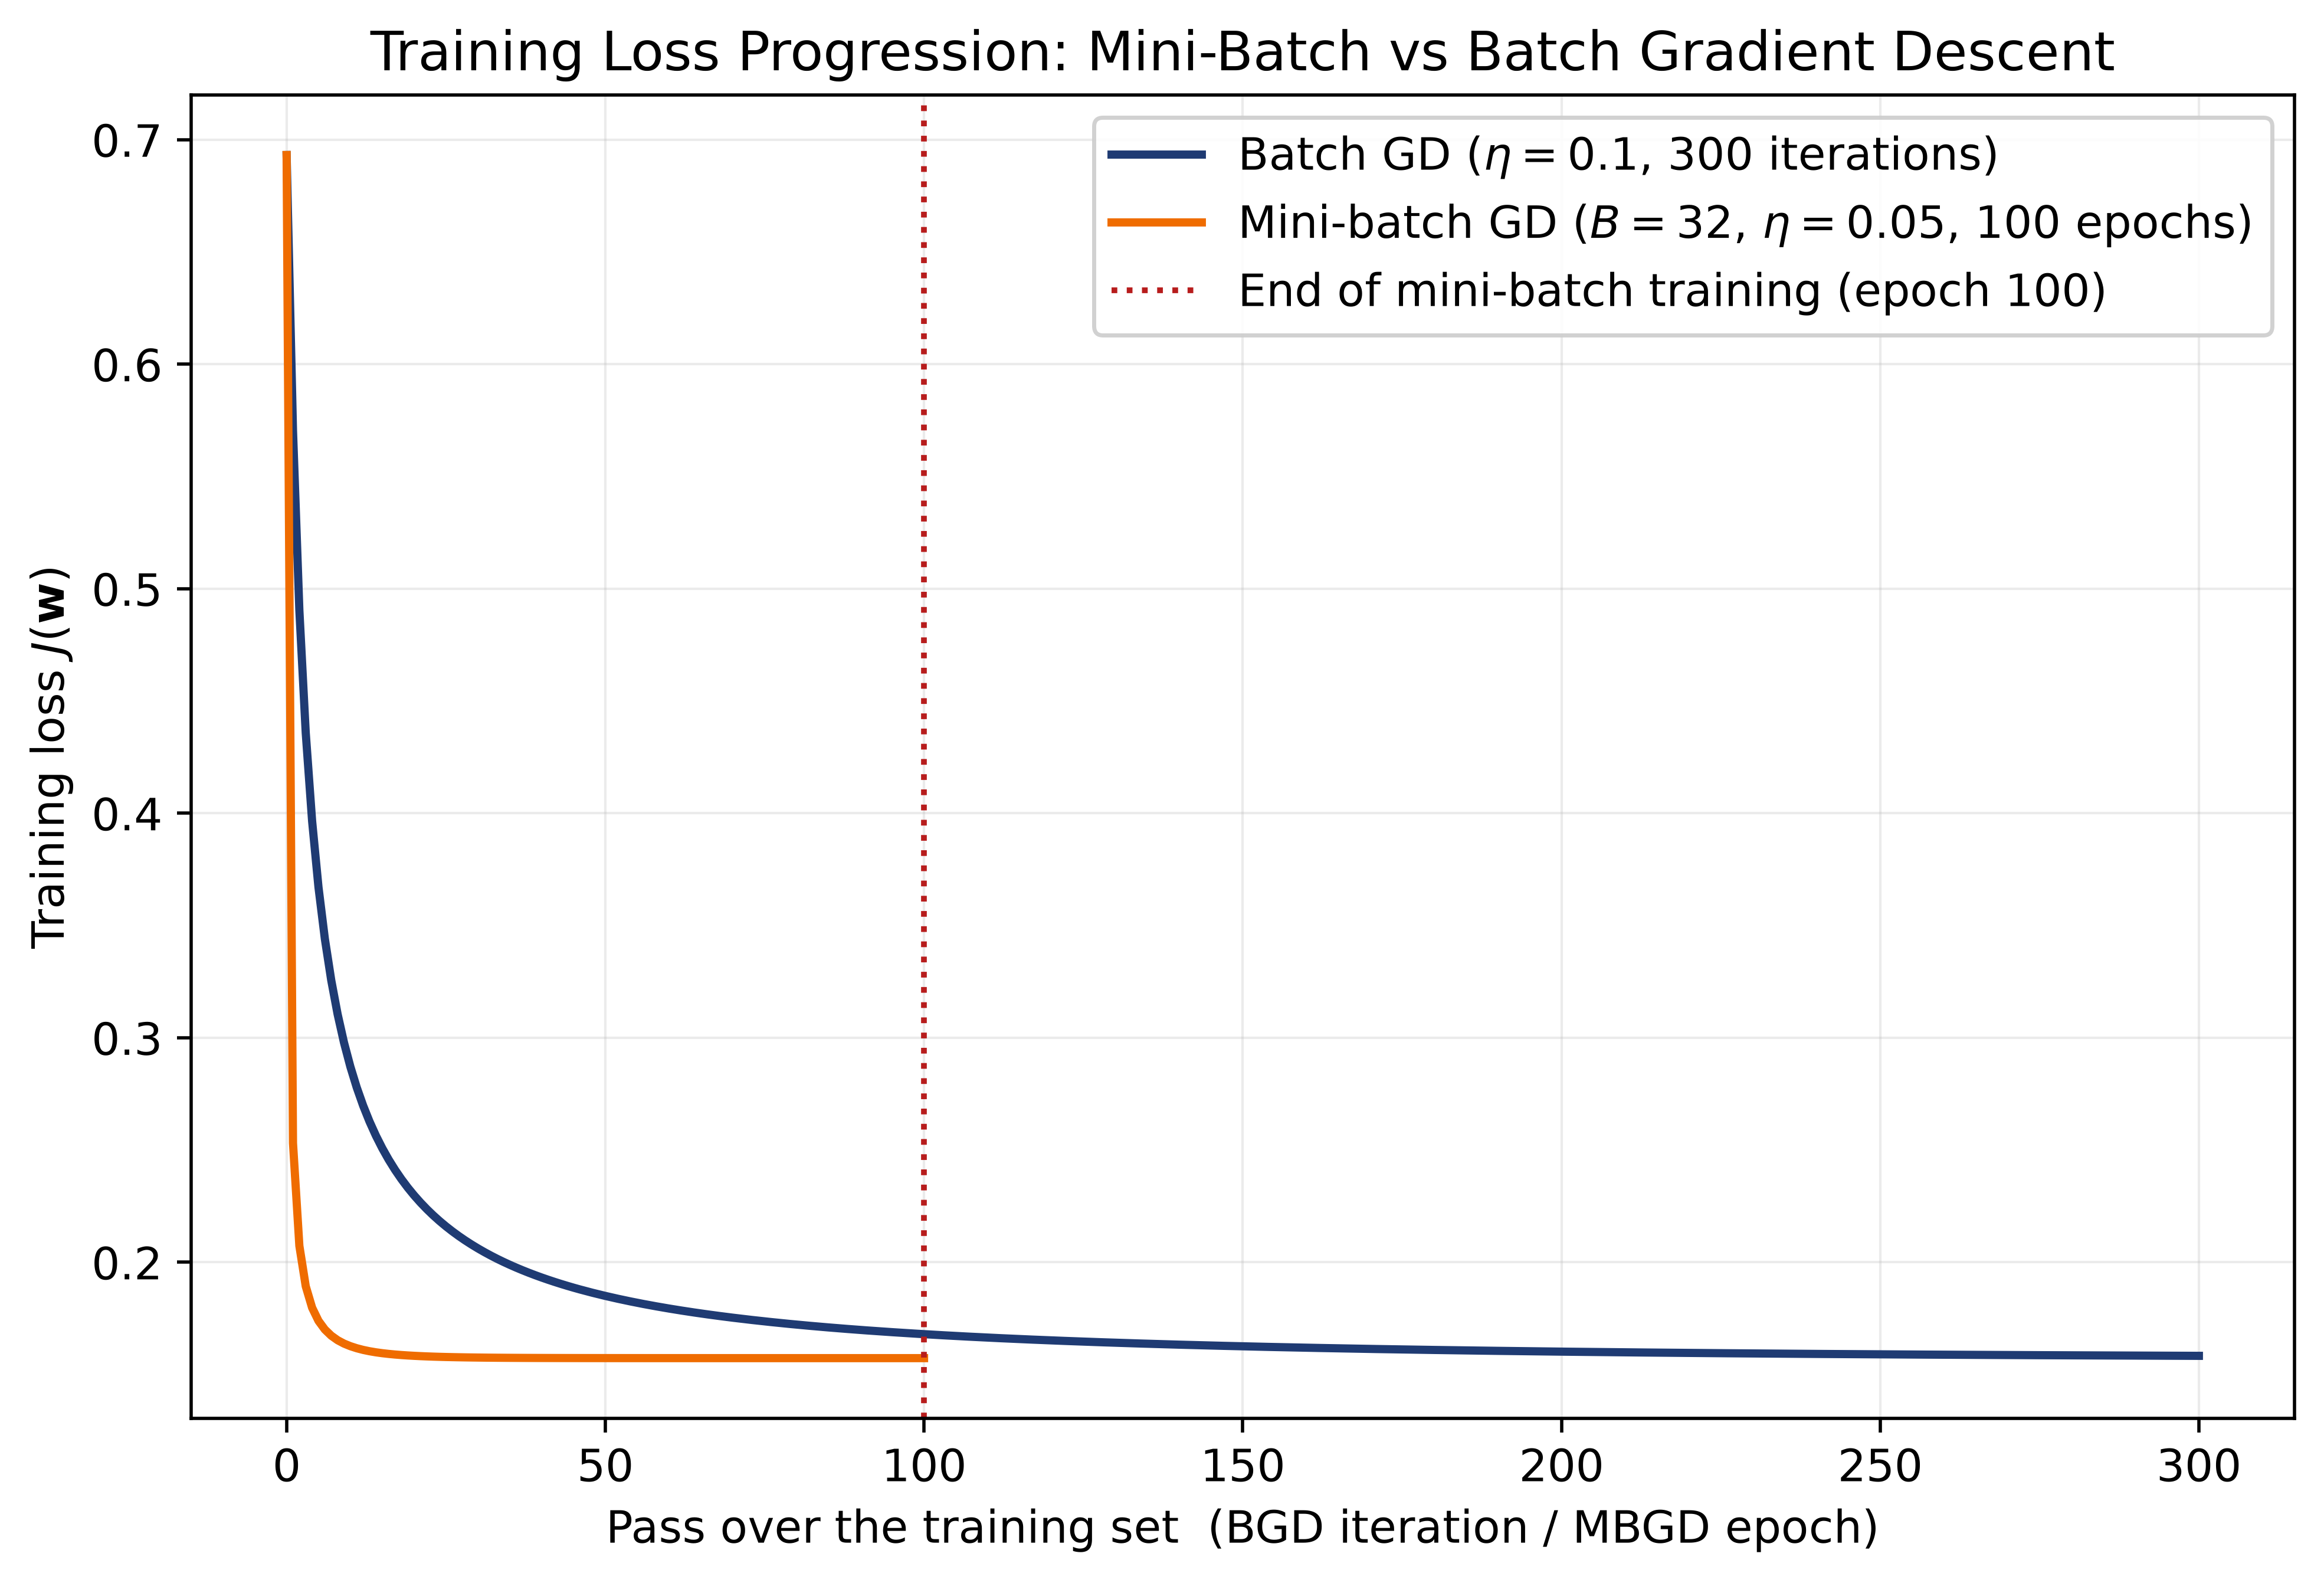
\includegraphics[width=0.88\textwidth]{figures/q3_4_minibatch.png}
\caption{Training loss progression of mini-batch gradient descent against batch gradient descent.
One batch iteration and one mini-batch epoch each cost a single pass over the training set.}
\label{fig:mbgd}
\end{figure}

\textbf{Results}

\begin{table}[H]
\centering
\caption{Mini-batch gradient descent with $B = 32$, $\eta = 0.05$ and $E = 100$ epochs.}
\label{tab:mbgd}
\begin{tabular}{lc}
\toprule
\textbf{Quantity} & \textbf{Value} \\
\midrule
Batch size $B$              & 32 (30 updates per epoch) \\
Learning rate $\eta$        & 0.05 \\
Epochs $E$                  & 100 \\
Final weights $\mathbf{w}$  & $[-0.024086,\; 1.966431,\; 0.789966]$ \\
Final loss $J_E$            & $0.157281$ \\
Test accuracy               & $0.9333$ \\
\bottomrule
\end{tabular}
\end{table}

Mini-batch gradient descent performs 30 parameter updates in every epoch, because the 960 training
samples are divided into batches of 32. Batch gradient descent performs only one update for each
pass over the data.

Both methods use the whole training set once per step on the $x$-axis of the plot, so the
comparison is fair in terms of computation. After 100 passes, mini-batch reaches a loss of
$0.157281$, while batch gradient descent is still at $0.167955$. Even after all 300 of its
iterations, batch gradient descent only reaches $0.158305$.

So mini-batch gradient descent makes much faster progress per pass over the data. This happens
because it updates the weights 30 times in each epoch instead of once, so the weights move much
further for the same amount of computation.

The mini-batch curve is slightly noisy because each update uses only 32 samples, so its gradient is
an estimate of the true gradient rather than the exact value. Here the noise is small and the loss
still decreases smoothly. The indices are reshuffled at the start of every epoch so the batches are
different each time, which stops the model from repeating the same sequence of updates.

\subsection{Damped Newton's Method}

\qtext{Implement damped Newton's optimization method using the update step
$\mathbf{w}^{(t+1)} \leftarrow \mathbf{w}^{(t)} -
(\mathbf{H} + 10^{-6}\mathbf{I})^{-1}\nabla J(\mathbf{w}^{(t)})$, where $10^{-6}\mathbf{I}$
guarantees numerical invertibility. Train for at most 20 iterations using the same early stopping
condition. Use \texttt{np.linalg.solve} to directly compute search directions rather than
computing explicit matrix inverses.}

\lstinputlisting[caption={Damped Newton's method using \texttt{np.linalg.solve} for the search
direction.}, label={lst:newton}]{code/3_5_newton.py}

\begin{lstlisting}[style=plainout]
Final weights    : w0 = -0.024093, w1 = 1.968123, w2 = 0.790651
Iterations       : 8
Early stopped    : True   (|J_t - J_t-1| = 3.059e-14)
Final loss J_T   : 0.15728072
Test accuracy    : 0.9333
\end{lstlisting}

\begin{table}[H]
\centering
\caption{Damped Newton's method against batch gradient descent on the same training set.}
\label{tab:newton}
\begin{tabular}{lcc}
\toprule
\textbf{Quantity} & \textbf{Batch GD} & \textbf{Newton} \\
\midrule
Iterations       & 300 (capped) & 8 (converged) \\
$|J_t - J_{t-1}|$ at stop & $1.000\times10^{-5}$ & $3.059\times10^{-14}$ \\
Final loss $J_T$ & 0.15830462 & 0.15728072 \\
Test accuracy    & 0.9333 & 0.9333 \\
\bottomrule
\end{tabular}
\end{table}

\subsection{Convergence Comparison}

\qtext{Plot loss versus iteration for both Batch Gradient Descent and Newton's Method on a single
logarithmic-scale plot. Compare convergence velocity (number of iterations), computational
complexity per step ($\mathcal{O}(ND)$ vs.\ $\mathcal{O}(ND^2 + D^3)$), and numerical stability.}

\lstinputlisting[caption={Loss against iteration for both optimizers on a logarithmic scale.},
                 label={lst:conv}]{code/3_6_plot.py}

\begin{figure}[H]
\centering
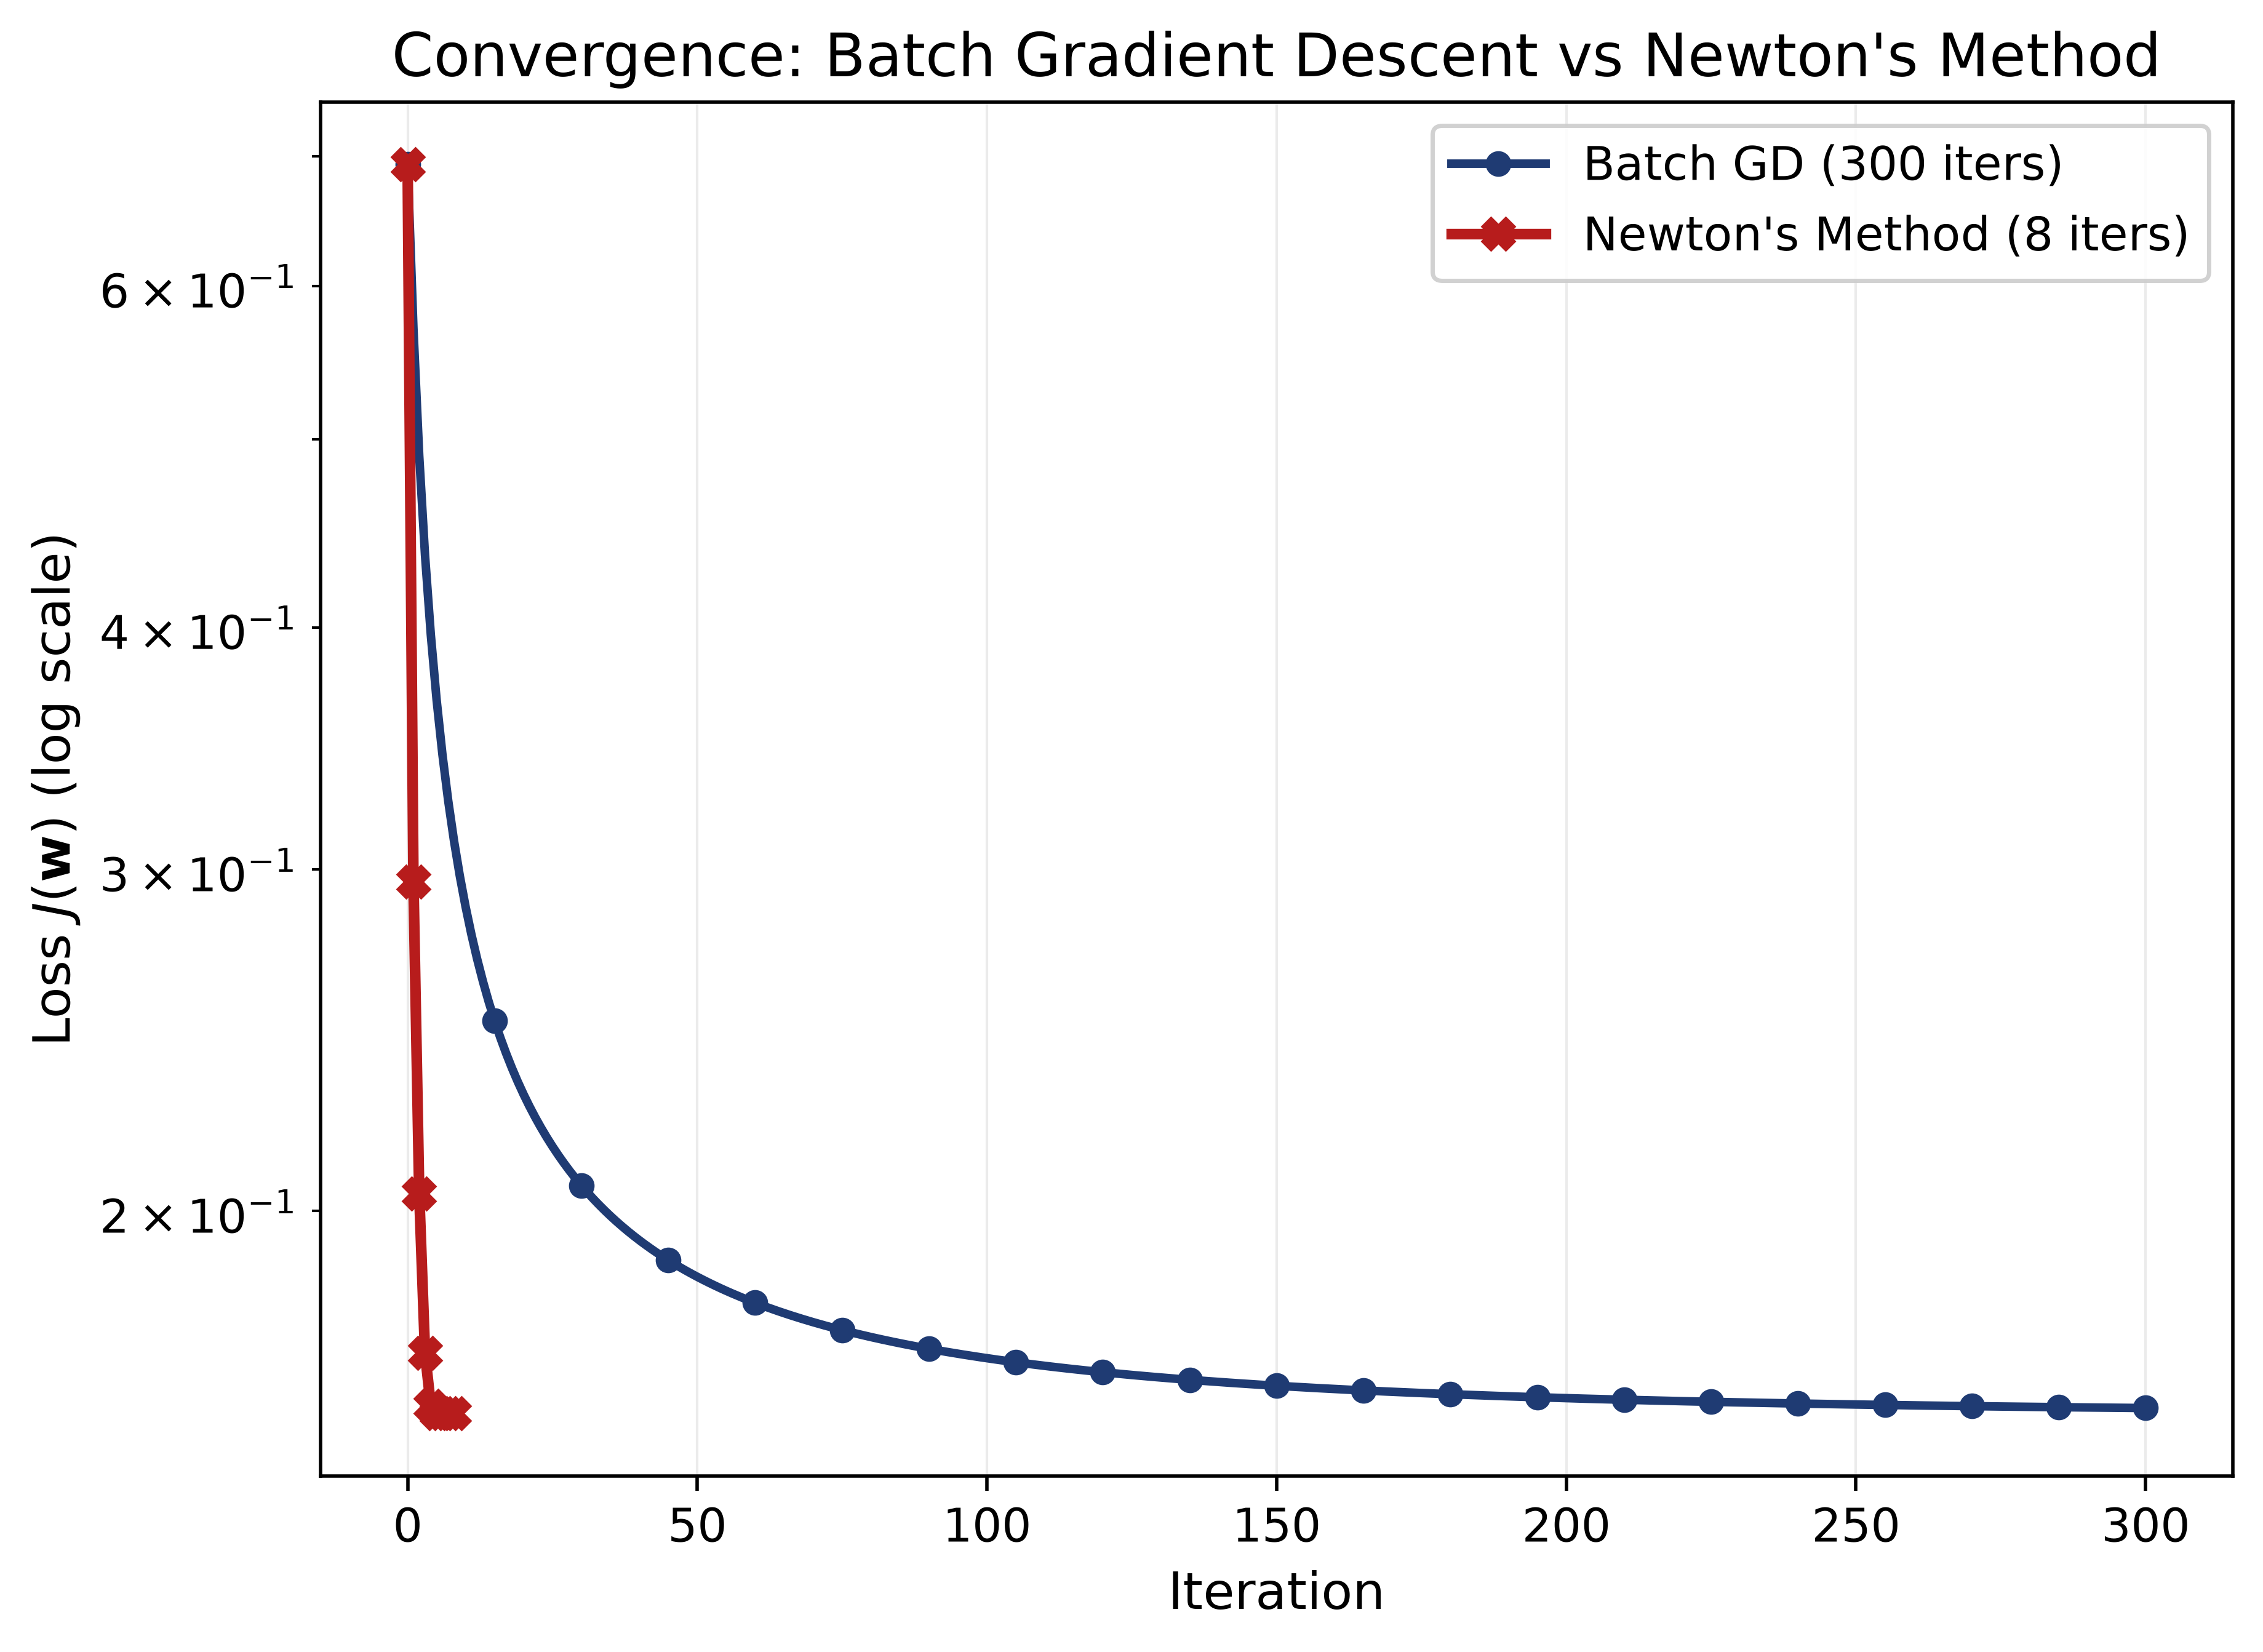
\includegraphics[width=0.86\textwidth]{figures/q3_6_convergence.png}
\caption{Convergence of batch gradient descent against damped Newton's method, loss on a
logarithmic scale.}
\label{fig:conv}
\end{figure}

\textbf{Convergence speed}

On the log-scale plot, Newton's method drops to the minimum in only a few iterations
($\sim$5), while Batch GD needs all 300 iterations and still does not reach the $10^{-8}$
tolerance. Newton's method uses the Hessian (curvature), so it converges quadratically near the
optimum, whereas GD is a slow first-order method.

\textbf{Complexity per step}

A GD step only needs the gradient, $\mathcal{O}(ND)$. A Newton step needs the Hessian,
$\mathcal{O}(ND^2)$, plus solving the linear system, $\mathcal{O}(D^3)$. Since $D = 2$ here this is
negligible and Newton wins overall, but for large $D$ the $D^3$ term would make Newton too
expensive and GD preferable.

\textbf{Numerical stability}

When $p_i \to 0$ or $1$, the terms $p_i(1-p_i) \to 0$, so $\mathbf{H}$ can become nearly singular.
The damping term $10^{-6}\mathbf{I}$ keeps it positive definite so \texttt{np.linalg.solve} stays
stable. GD never inverts a matrix, so it avoids this issue, but it struggles on ill-conditioned
loss surfaces.

\subsection{Effect of Feature Scaling on Conditioning}

\qtext{Multiply the second feature of $\mathbf{X}$ by 100 ($x_2 \leftarrow 100 \cdot x_2$) without
standardizing features. Run Batch Gradient Descent on this unscaled dataset. Explain why the loss
oscillates or fails to converge, referencing the condition number
$\kappa(\mathbf{H}) = \frac{\lambda_{\max}}{\lambda_{\min}}$ of the loss surface Hessian. Propose
two concrete remedies.}

\lstinputlisting[caption={Batch gradient descent on the badly scaled dataset, with the Hessian
condition number before and after scaling.}, label={lst:scaling}]{code/3_7_scaling.py}

\begin{lstlisting}[style=plainout]
kappa(H) unscaled : 9.0
kappa(H) x2*100   : 3.6e+04

first 10 losses: [  0.693 127.459  36.296 207.473 291.215 200.05  108.885  17.734 276.153
 272.708]
final loss      : 1.834e+02
test accuracy   : 0.6833
\end{lstlisting}

Scaling $x_2 \leftarrow 100\,x_2$ multiplies the curvature of the loss along $w_2$ by about
$100^2$, so the Hessian eigenvalues spread apart:
$\kappa(\mathbf{H}) = \lambda_{\max}/\lambda_{\min}$ jumps from $\mathcal{O}(10)$ (unscaled) to
$\mathcal{O}(10^5)$, and the level sets become long, narrow valleys. Gradient descent with fixed
$\eta$ is stable only when $\eta < 2/\lambda_{\max}$; here $\eta\,\lambda_{\max} \gg 2$, so each
update along $w_2$ overshoots the valley, and the loss oscillates / diverges instead of converging
(seen in the printed losses). Even a smaller, stable $\eta$ would make progress along the shallow
direction impractically slow.

\textbf{Two remedies:}
\begin{enumerate}
\item \textbf{Standardize the features} ($z = (x-\mu)/\sigma$) so all directions have comparable
curvature ($\kappa \approx 1$); then one $\eta$ converges smoothly.
\item \textbf{Use a scale-invariant second-order method} --- (damped) Newton's method
preconditions the gradient with $\mathbf{H}^{-1}$, cancelling the curvature imbalance (an adaptive
method such as Adam, or a much smaller $\eta$, also works).
\end{enumerate}

\end{document}
